\documentclass{article}\usepackage[]{graphicx}\usepackage[]{color}
%% maxwidth is the original width if it is less than linewidth
%% otherwise use linewidth (to make sure the graphics do not exceed the margin)
\makeatletter
\def\maxwidth{ %
  \ifdim\Gin@nat@width>\linewidth
    \linewidth
  \else
    \Gin@nat@width
  \fi
}
\makeatother

\definecolor{fgcolor}{rgb}{0.345, 0.345, 0.345}
\newcommand{\hlnum}[1]{\textcolor[rgb]{0.686,0.059,0.569}{#1}}%
\newcommand{\hlstr}[1]{\textcolor[rgb]{0.192,0.494,0.8}{#1}}%
\newcommand{\hlcom}[1]{\textcolor[rgb]{0.678,0.584,0.686}{\textit{#1}}}%
\newcommand{\hlopt}[1]{\textcolor[rgb]{0,0,0}{#1}}%
\newcommand{\hlstd}[1]{\textcolor[rgb]{0.345,0.345,0.345}{#1}}%
\newcommand{\hlkwa}[1]{\textcolor[rgb]{0.161,0.373,0.58}{\textbf{#1}}}%
\newcommand{\hlkwb}[1]{\textcolor[rgb]{0.69,0.353,0.396}{#1}}%
\newcommand{\hlkwc}[1]{\textcolor[rgb]{0.333,0.667,0.333}{#1}}%
\newcommand{\hlkwd}[1]{\textcolor[rgb]{0.737,0.353,0.396}{\textbf{#1}}}%

\usepackage{framed}
\makeatletter
\newenvironment{kframe}{%
 \def\at@end@of@kframe{}%
 \ifinner\ifhmode%
  \def\at@end@of@kframe{\end{minipage}}%
  \begin{minipage}{\columnwidth}%
 \fi\fi%
 \def\FrameCommand##1{\hskip\@totalleftmargin \hskip-\fboxsep
 \colorbox{shadecolor}{##1}\hskip-\fboxsep
     % There is no \\@totalrightmargin, so:
     \hskip-\linewidth \hskip-\@totalleftmargin \hskip\columnwidth}%
 \MakeFramed {\advance\hsize-\width
   \@totalleftmargin\z@ \linewidth\hsize
   \@setminipage}}%
 {\par\unskip\endMakeFramed%
 \at@end@of@kframe}
\makeatother

\definecolor{shadecolor}{rgb}{.97, .97, .97}
\definecolor{messagecolor}{rgb}{0, 0, 0}
\definecolor{warningcolor}{rgb}{1, 0, 1}
\definecolor{errorcolor}{rgb}{1, 0, 0}
\newenvironment{knitrout}{}{} % an empty environment to be redefined in TeX

\usepackage{alltt}

\usepackage{hyperref}

\def\code#1{\texttt{#1}}
\IfFileExists{upquote.sty}{\usepackage{upquote}}{}

\begin{document}

\title{bfastSpatial}
\author{Lo\"{i}c Dutrieux, Ben DeVries, Jan Verbesselt}

\maketitle

\section{Preamble}
The \code{bfastSpatial} provides utilities to performs change detection analysis on time-series of spatial gridded data, such as time-series of remote sensing images (Landsat, MODIS and the likes). The tools provided by \code{bfastSpatial} allows a user to perform all the steps of the change detection workflow, from pre-processing raw surface reflectance Landsat data, inventorying and preparing them for analysis to the production and formatting of change detection results. The present document aims at providing guidance to the users of \code{bfastSpatial} by detailing every steps of the process.

\section{Set up your system}
\subsection{Windows}
There are no specific system requirements for Windows, besides having (a recent version of) R installed; installing the \code{bfastSpatial} package will automatically install the required dependencies.  
\subsection{Linux \& Mac}
Some pre-processing functions require the \code{rgdal} package, which is a binding between the gdal library and R. For \code{rgdal} to work on Linux and Mac systems, gdal should be installed and properly set-up. For that, please refer to the web page of the \href{http://www.gdal.org/}{gdal project} as well as \href{http://cran.r-project.org/web/packages/rgdal/index.html}{rgdal}.

\section{Downloading Landsat data from Earth Explorer}
Working with Landsat time-series often involves downloading large amounts of data. The full Landsat archive for one path/row may very well exceed 500 scenes in some parts of the world. The most common way to access the data is via the \href{http://earthexplorer.usgs.gov/}{Earth Explorer platform}. You need to have an account before being able to request data to be pre-processed.
\subsection{Placing your order}
USGS is planning to support the delivery of data in different formats (HDF, GeoTiff, binary). GeoTiff is a common and easy to handle format of raster data and should be your preferred choice if you are working in Windows.
\subsection{Downloading the data}
Once you receive the e-mail from USGS notifying you that your order has been pre-processed, you will be able to proceed to the download of the data. Because the amount of scenes is usually large, the use of a download manager is highly recommended. Two options:
\begin{itemize}
\item The Bulk Download Application
\item The DownloadThemAll plugin of the firefox browser
\end{itemize}




\section{Data pre-processing}
The \code{bfastSpatial} package includes utilities to pre-process Landsat surface reflectance data and prepare them for subsequent analysis with the change detection functions such as \code{bfmSpatial}. The overall Landsat pre-processing requires to:
\begin{itemize}
\item Extract data from the tar.gz archive
\item Calculate Vegetation Indices from surface reflectance bands (when not provided by USGS)
\item Crop the data to a desired spatial extent
\item Apply one of the cloud/land mask supplied with the data
\item Create a the spatio-temporal object to be used in subsequent analyses
\end{itemize}

The two important functions to perform the above mentioned steps are \code{processLandsat} and \code{processLandsatBatch}. The former is a wrapper that performs the above steps sequentially, automatically generating file names and deleting unnecessary intermediary outputs. The latter (\code{processLandsatBatch}) allows a user to run \code{processLandsat} in batch mode, over several scenes, with parallel support. Several vegetation indices are supported by both \code{processLandsat} and \code{processLandsatBatch}.
Let's illustrate that with an example. We added subsets of Landsat data to the package in order to illustrate the pre-processing steps. The test datasets are stored under the \code{external/} directory of the installed package. To list the content of that directory, run the following comand.
\begin{knitrout}
\definecolor{shadecolor}{rgb}{0.969, 0.969, 0.969}\color{fgcolor}\begin{kframe}
\begin{alltt}
\hlkwd{list.files}\hlstd{(}\hlkwd{system.file}\hlstd{(}\hlstr{"external"}\hlstd{,} \hlkwc{package} \hlstd{=} \hlstr{"bfastSpatial"}\hlstd{),} \hlkwc{full.names} \hlstd{=} \hlnum{TRUE}\hlstd{)}
\end{alltt}
\begin{verbatim}
## [1] "/home/dutri001/R/x86_64-pc-linux-gnu-library/3.1/bfastSpatial/external/LE72220622001176EDC01.tar.gz"
## [2] "/home/dutri001/R/x86_64-pc-linux-gnu-library/3.1/bfastSpatial/external/LE72220622002147EDC00.tar.gz"
## [3] "/home/dutri001/R/x86_64-pc-linux-gnu-library/3.1/bfastSpatial/external/LT52220622004289CUB01.tar.gz"
\end{verbatim}
\end{kframe}
\end{knitrout}

Using the \code{full.names=TRUE} argument allows you to directly use the elements of the list create without having to set working directories.

% TODO add example here

Once the vegetation index layers have been produced for several dates, they can be stacked, in order to create a multilayer raster object, with time dimention written in the file as well. The function to perform this operation on Landsat data is the \code{timeStack} function. By simply providing a list of file names or a directory containing the files, the function will create a multilayer object and directly parse through the file names to extract temporal information from them and write that information to the object created.

% TODO add timeStack example here



\section{Data Inventory}

A number of functions are available in the bfastSpatial package to help keep an inventory of data in a raster time series stack. These functions range from basic scene information (\code{getSceneinfo()}) to summary of pixel values per year in the time series (\code{annualSummary()}).

The following functions are included in the Data Inventory module:
\begin{enumerate}
\item \code{getSceneinfo()}
\item \code{countObs()}
\item \code{summaryBrick()}
\item \code{annualSummary()}
\end{enumerate}

\subsection{Basic Scene Information: \code{getSceneinfo()}}

\code{getSceneinfo()} allows the user to list the information contained within a scene ID. Currently, only Landsat scene ID's are supported. For example, the scene ID ``LE71700552007309ASN00" tells us that the scene is from the Landsat 7 ETM+ sensor ('LE7'), path-row 170-55 ('170055') and was acquired on the 309th day of the year 2007 ('2007309'). Calling \code{getSceneinfo('LE71700552007309ASN00')} will give a data.frame with one row showing all of this information.

\begin{knitrout}
\definecolor{shadecolor}{rgb}{0.969, 0.969, 0.969}\color{fgcolor}\begin{kframe}
\begin{alltt}
\hlkwd{getSceneinfo}\hlstd{(}\hlstr{"LE71700552007309ASN00"}\hlstd{)}
\end{alltt}
\begin{verbatim}
##                        sensor path row       date
## LE71700552007309 ETM+ SLC-off  170  55 2007-11-05
\end{verbatim}
\end{kframe}
\end{knitrout}


When working with Landsat data, it is a good idea to assign and keep these sceneID's as layer names (see \code{?raster::names}) so the relevant information is associated to each raster layer.

\begin{knitrout}
\definecolor{shadecolor}{rgb}{0.969, 0.969, 0.969}\color{fgcolor}\begin{kframe}
\begin{alltt}
\hlcom{# show scene info from tura layers}
\hlkwd{data}\hlstd{(tura)}
\hlkwd{head}\hlstd{(}\hlkwd{names}\hlstd{(tura))}
\end{alltt}
\begin{verbatim}
## [1] "LE71700551999255AGS00" "LE71700551999271EDC00" "LE71700552000114SGS00"
## [4] "LE71700552000194EDC00" "LE71700552000258SGS00" "LE71700552001036SGS00"
\end{verbatim}
\begin{alltt}
\hlstd{s} \hlkwb{<-} \hlkwd{getSceneinfo}\hlstd{(}\hlkwd{names}\hlstd{(tura))}
\hlkwd{head}\hlstd{(s)}
\end{alltt}
\begin{verbatim}
##                       sensor path row       date
## LE71700551999255 ETM+ SLC-on  170  55 1999-09-12
## LE71700551999271 ETM+ SLC-on  170  55 1999-09-28
## LE71700552000114 ETM+ SLC-on  170  55 2000-04-23
## LE71700552000194 ETM+ SLC-on  170  55 2000-07-12
## LE71700552000258 ETM+ SLC-on  170  55 2000-09-14
## LE71700552001036 ETM+ SLC-on  170  55 2001-02-05
\end{verbatim}
\begin{alltt}
\hlcom{# add a column for years and plot # of scenes per year}
\hlstd{s}\hlopt{$}\hlstd{year} \hlkwb{<-} \hlkwd{as.numeric}\hlstd{(}\hlkwd{substr}\hlstd{(s}\hlopt{$}\hlstd{date,} \hlnum{1}\hlstd{,} \hlnum{4}\hlstd{))}
\hlkwd{hist}\hlstd{(s}\hlopt{$}\hlstd{year,} \hlkwc{breaks} \hlstd{=} \hlkwd{c}\hlstd{(}\hlnum{1984}\hlopt{:}\hlnum{2014}\hlstd{),} \hlkwc{main} \hlstd{=} \hlstr{"p170r55: Scenes per Year"}\hlstd{,} \hlkwc{xlab} \hlstd{=} \hlstr{"year"}\hlstd{,}
    \hlkwc{ylab} \hlstd{=} \hlstr{"# of scenes"}\hlstd{)}
\end{alltt}
\end{kframe}
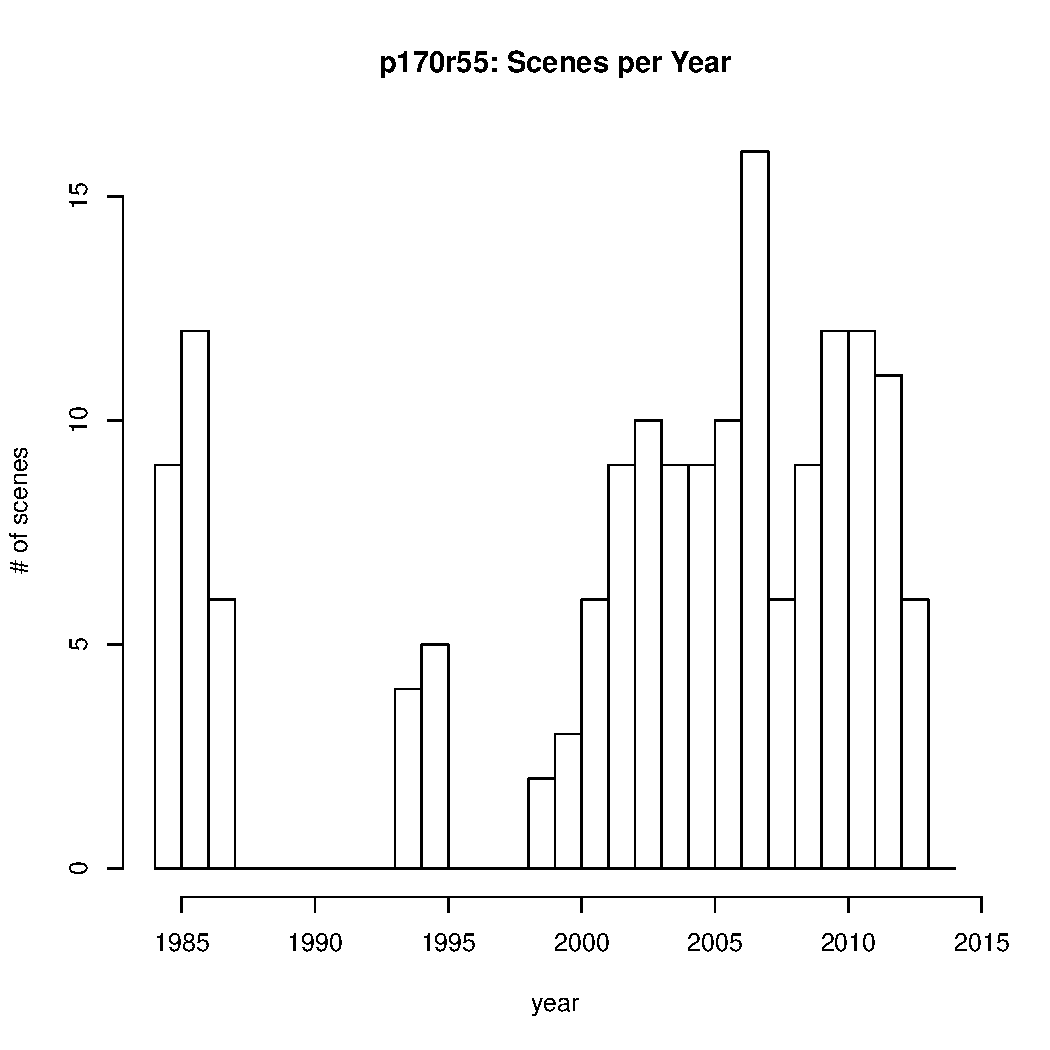
\includegraphics[width=\maxwidth]{figure/getSceneinfo-tura} 

\end{knitrout}


We can combine the dates and sensor information to get more of an idea of where our data are coming from.

\begin{knitrout}
\definecolor{shadecolor}{rgb}{0.969, 0.969, 0.969}\color{fgcolor}\begin{kframe}
\begin{alltt}
\hlkwd{library}\hlstd{(ggplot2)}
\hlstd{p} \hlkwb{<-} \hlkwd{ggplot}\hlstd{(}\hlkwc{data} \hlstd{= s,} \hlkwd{aes}\hlstd{(}\hlkwc{x} \hlstd{= year))}
\hlstd{p} \hlkwb{<-} \hlstd{p} \hlopt{+} \hlkwd{geom_bar}\hlstd{(}\hlkwd{aes}\hlstd{(}\hlkwc{fill} \hlstd{= sensor),} \hlkwc{binwidth} \hlstd{=} \hlnum{1}\hlstd{,} \hlkwc{col} \hlstd{=} \hlstr{"black"}\hlstd{)}
\hlstd{p} \hlkwb{<-} \hlstd{p} \hlopt{+} \hlkwd{labs}\hlstd{(}\hlkwc{y} \hlstd{=} \hlstr{"number of scenes"}\hlstd{)}
\hlstd{p}
\end{alltt}
\end{kframe}
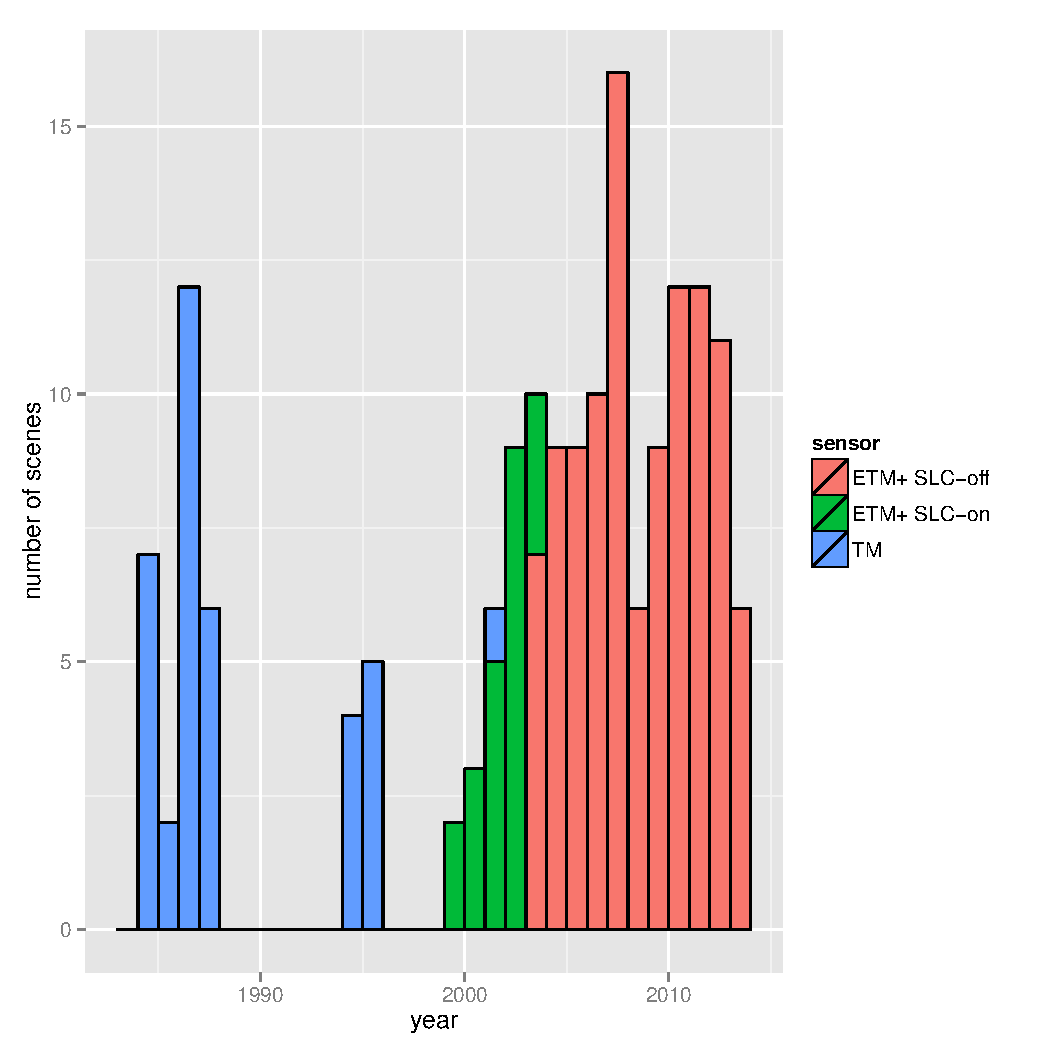
\includegraphics[width=\maxwidth]{figure/getSceneinfo-ggplot} 

\end{knitrout}


More examples can be found under \code{?getSceneinfo}. Many other functions in the bfastSpatial package rely on getSceneinfo to extract relevant scene information, such as acquisition dates to be passed to \code{bfmSpatial()} or \code{bfmPixel()}.

\subsection{Valid Observations: \code{countObs()}}

The number of available observations in a raster time series can be calculated by using countObs(). This function "drills" through pixels of a time series and counts the number of pixels with a non-NA value. Optionally, any other value can be supplied as a substitute for NA (e.g. the number of non-zero values per pixel can also be queried).

\begin{knitrout}
\definecolor{shadecolor}{rgb}{0.969, 0.969, 0.969}\color{fgcolor}\begin{kframe}
\begin{alltt}
\hlkwd{data}\hlstd{(tura)}
\hlstd{obs} \hlkwb{<-} \hlkwd{countObs}\hlstd{(tura)}
\hlkwd{plot}\hlstd{(obs)}
\end{alltt}
\end{kframe}
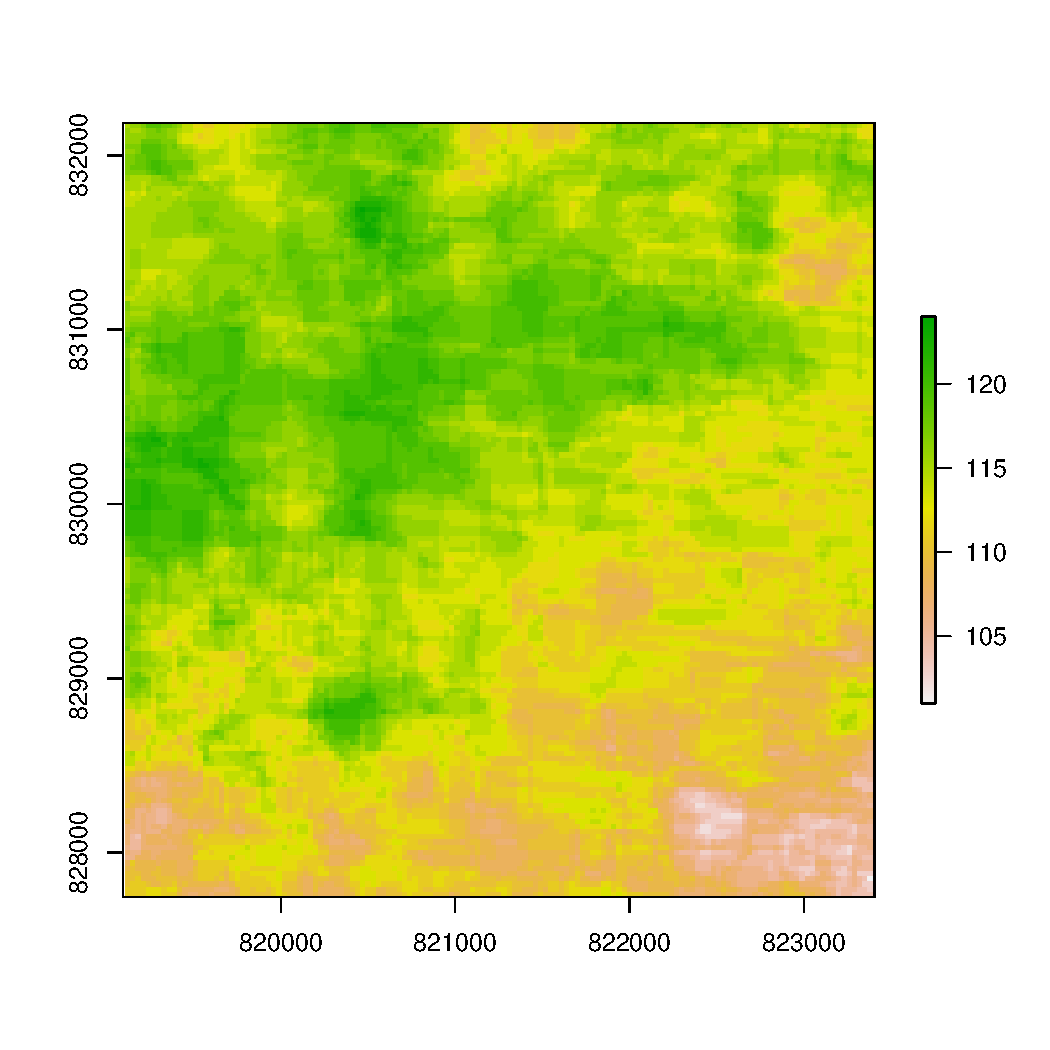
\includegraphics[width=\maxwidth]{figure/countObs} 
\begin{kframe}\begin{alltt}
\hlkwd{summary}\hlstd{(obs)}
\end{alltt}
\begin{verbatim}
##         layer
## Min.      101
## 1st Qu.   112
## Median    114
## 3rd Qu.   117
## Max.      124
## NA's        0
\end{verbatim}
\end{kframe}
\end{knitrout}


Values can also be expressed as a percentage if \code{as.perc} is set to \code{TRUE}.

\begin{knitrout}
\definecolor{shadecolor}{rgb}{0.969, 0.969, 0.969}\color{fgcolor}\begin{kframe}
\begin{alltt}
\hlcom{# valid observations}
\hlstd{obs} \hlkwb{<-} \hlkwd{countObs}\hlstd{(tura,} \hlkwc{as.perc} \hlstd{=} \hlnum{TRUE}\hlstd{)}
\hlkwd{summary}\hlstd{(obs)}
\end{alltt}
\begin{verbatim}
##         layer
## Min.    60.84
## 1st Qu. 67.47
## Median  68.67
## 3rd Qu. 70.48
## Max.    74.70
## NA's     0.00
\end{verbatim}
\begin{alltt}
\hlcom{# \textbackslash{}% NA per pixel}
\hlstd{percNA} \hlkwb{<-} \hlnum{100} \hlopt{-} \hlkwd{countObs}\hlstd{(tura,} \hlkwc{as.perc} \hlstd{=} \hlnum{TRUE}\hlstd{)}
\hlkwd{plot}\hlstd{(percNA,} \hlkwc{main} \hlstd{=} \hlstr{"percent NA per pixel"}\hlstd{)}
\end{alltt}
\end{kframe}
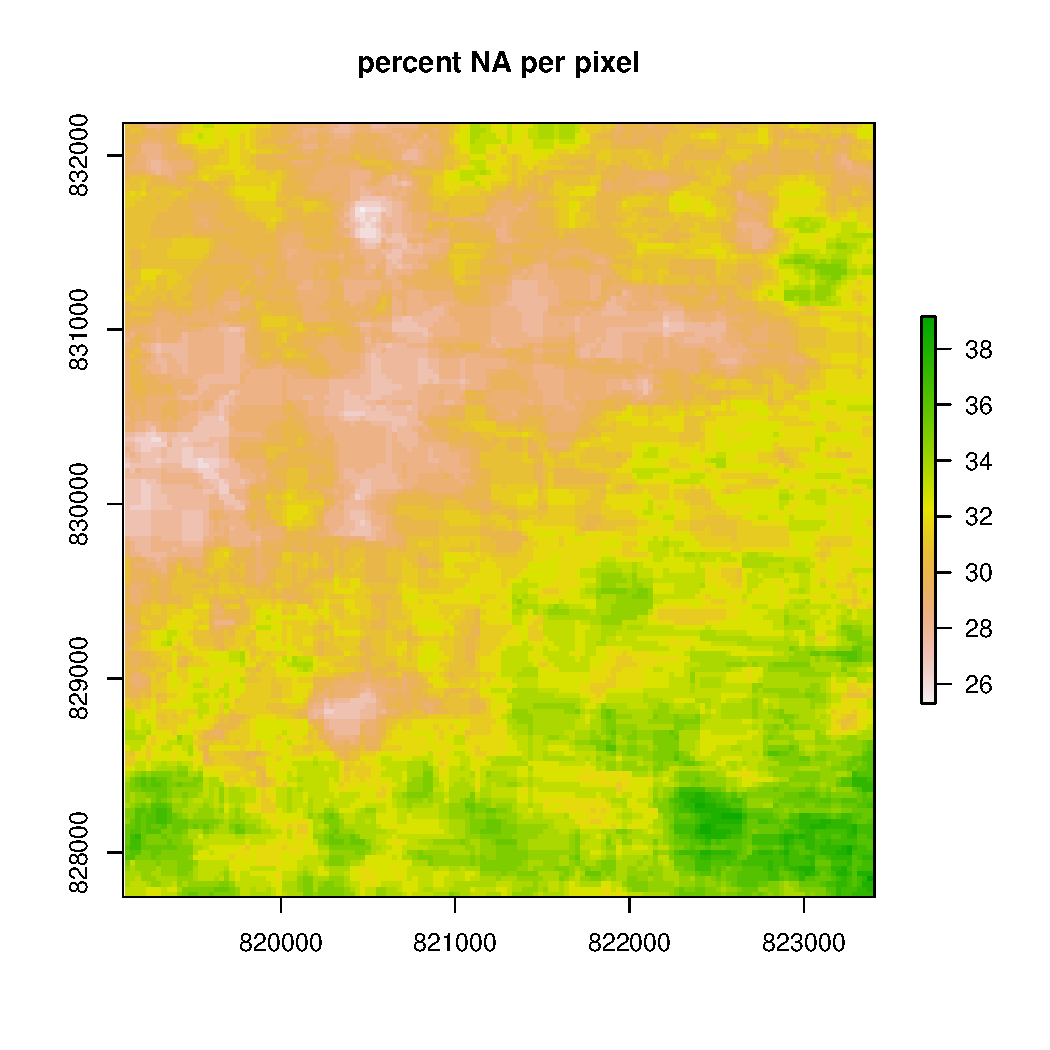
\includegraphics[width=\maxwidth]{figure/countObs-asperc} 
\begin{kframe}\begin{alltt}
\hlkwd{summary}\hlstd{(percNA)}
\end{alltt}
\begin{verbatim}
##         layer
## Min.    25.30
## 1st Qu. 29.52
## Median  31.33
## 3rd Qu. 32.53
## Max.    39.16
## NA's     0.00
\end{verbatim}
\end{kframe}
\end{knitrout}


\subsection{Summary Statistics: \code{summaryBrick()} and \code{annualSummary()}}

In this section, we will calculate summary statistics for the Tura RasterBrick. First, general statistics for the entire brick can be calculated using \code{summaryBrick()}. In fact, \code{countObs()} is essentially a specific version of \code{summaryBrick}. \code{summaryBrick()} takes a RasterBrick as its first argument and a function as its second argument, and all others are optional arguments. Calculating the mean of each pixel is simple.

\begin{knitrout}
\definecolor{shadecolor}{rgb}{0.969, 0.969, 0.969}\color{fgcolor}\begin{kframe}
\begin{alltt}
\hlstd{meanVI} \hlkwb{<-} \hlkwd{summaryBrick}\hlstd{(tura,} \hlkwc{fun} \hlstd{= mean)}  \hlcom{# na.rm=FALSE by default}
\hlkwd{plot}\hlstd{(meanVI)}
\end{alltt}
\end{kframe}
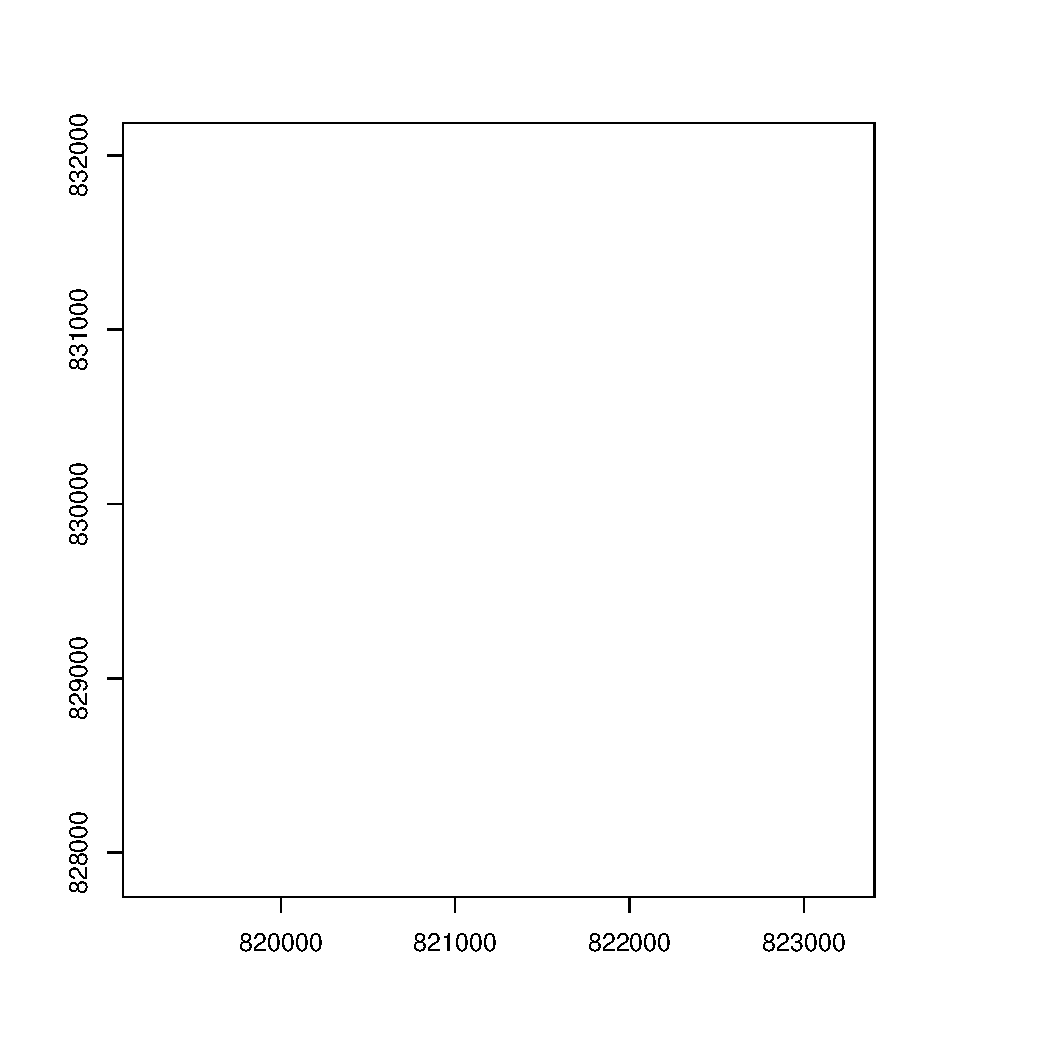
\includegraphics[width=\maxwidth]{figure/summaryBrick-functions} 

\end{knitrout}


The fact that there are no values in the result stems from the fact that an \code{na.rm} argument has not been supplied. By default, this is set to \code{NULL} to ensure that other functions that do not take an \code{na.rm} argument (like \code{length}, for example) can also be used as \code{fun}. Since there are many \code{NA} values scattered through our RasterBrick as a result of cloud masking, \code{na.rm} must be set to \code{TRUE} for functions like \code{mean}, \code{median} and other common stats functions.

\begin{knitrout}
\definecolor{shadecolor}{rgb}{0.969, 0.969, 0.969}\color{fgcolor}\begin{kframe}
\begin{alltt}
\hlstd{meanVI} \hlkwb{<-} \hlkwd{summaryBrick}\hlstd{(tura,} \hlkwc{fun} \hlstd{= mean,} \hlkwc{na.rm} \hlstd{=} \hlnum{TRUE}\hlstd{)}
\hlkwd{plot}\hlstd{(meanVI)}
\end{alltt}
\end{kframe}
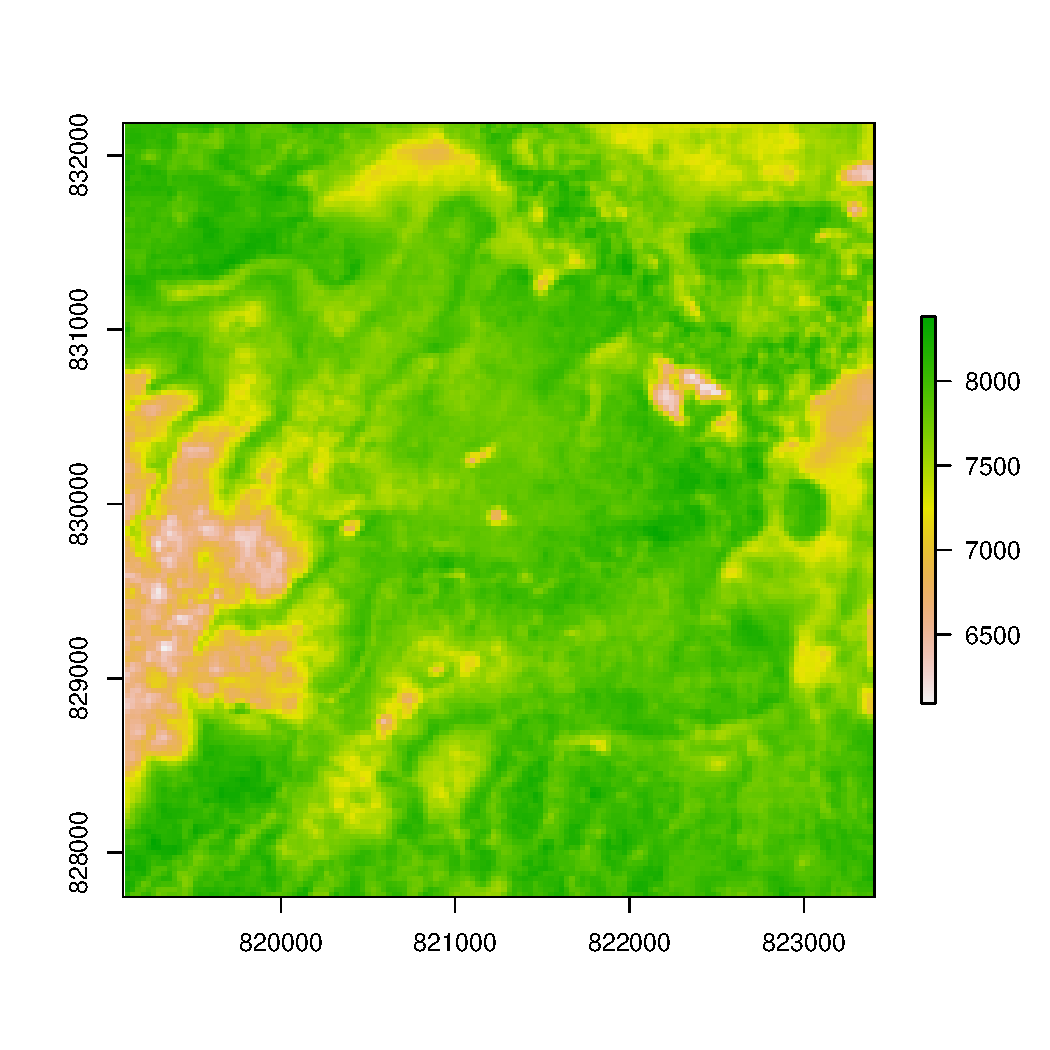
\includegraphics[width=\maxwidth]{figure/summaryBrick-narm} 

\end{knitrout}


\code{summaryBrick} can also take custom functions, provided these functinos are vectorized - in other words, they should be applicable to a vector extracted from a single pixel time series (for example, by taking a single cell number of the Tura RasterBrick: \code{x <- tura[500]}). Suppose we want to know how many observations per pixel exceed a certain threshold. First, we should define a function that can count the number of elements in a vector that exceed this threshold, and then pass this to \code{summaryBrick}. In this example, we will use 7000 as our threshold (remember that the values are scaled by 10000, so this corresponds to an NDVI of 0.7).

\begin{knitrout}
\definecolor{shadecolor}{rgb}{0.969, 0.969, 0.969}\color{fgcolor}\begin{kframe}
\begin{alltt}
\hlcom{# define a function that takes a vector as an argument}
\hlstd{checkThresh} \hlkwb{<-} \hlkwa{function}\hlstd{(}\hlkwc{x}\hlstd{) \{}
    \hlcom{# first, get rid of NA's}
    \hlstd{x} \hlkwb{<-} \hlstd{x[}\hlopt{!}\hlkwd{is.na}\hlstd{(x)]}
    \hlcom{# if there still values left, count how many are above the threshold}
    \hlcom{# otherwise, return a 0}
    \hlkwa{if} \hlstd{(}\hlkwd{length}\hlstd{(x)} \hlopt{>} \hlnum{0}\hlstd{) \{}
        \hlstd{y} \hlkwb{<-} \hlkwd{length}\hlstd{(x[x} \hlopt{>} \hlnum{7000}\hlstd{])}
    \hlstd{\}} \hlkwa{else} \hlstd{\{}
        \hlstd{y} \hlkwb{<-} \hlnum{0}
    \hlstd{\}}
    \hlcom{# return the value}
    \hlkwd{return}\hlstd{(y)}
\hlstd{\}}
\hlcom{# pass this functino to summaryBrick}
\hlstd{customStat} \hlkwb{<-} \hlkwd{summaryBrick}\hlstd{(tura,} \hlkwc{fun} \hlstd{= checkThresh)}
\hlkwd{plot}\hlstd{(customStat,} \hlkwc{main} \hlstd{=} \hlstr{"# of observations where NDVI > 0.7"}\hlstd{)}
\end{alltt}
\end{kframe}
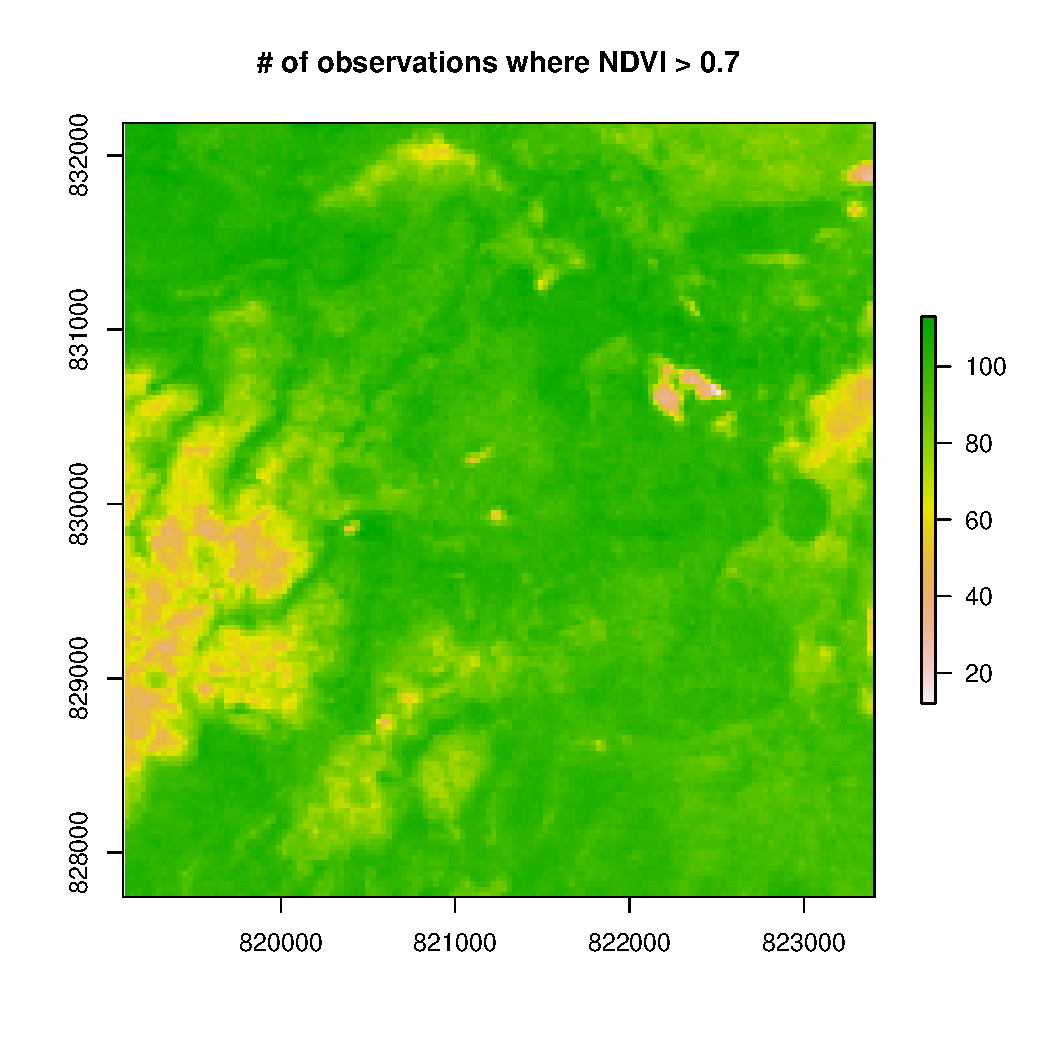
\includegraphics[width=\maxwidth]{figure/summaryBrick-custom} 

\end{knitrout}


Note that in this case we handled NA values within our function, so there was no need to specify a value for \code{na.rm}. \code{summaryBrick} has some optional arguments that allow constraints according to dates and sensor (currently only for Landsat data). \code{sensor} takes a character vector of sensors to constrain the data, while \code{minDate} and \code{maxDate} allow a date range to be set to constrain the data. In the following example, we will calculate median pixel values using different date and sensor ranges.

\begin{knitrout}
\definecolor{shadecolor}{rgb}{0.969, 0.969, 0.969}\color{fgcolor}\begin{kframe}
\begin{alltt}
\hlcom{# median values for all layers}
\hlstd{medVI} \hlkwb{<-} \hlkwd{summaryBrick}\hlstd{(tura,} \hlkwc{fun} \hlstd{= median,} \hlkwc{na.rm} \hlstd{=} \hlnum{TRUE}\hlstd{)}
\hlcom{# only ETM+ layers}
\hlstd{medVI_ETM} \hlkwb{<-} \hlkwd{summaryBrick}\hlstd{(tura,} \hlkwc{fun} \hlstd{= median,} \hlkwc{na.rm} \hlstd{=} \hlnum{TRUE}\hlstd{,} \hlkwc{sensor} \hlstd{=} \hlstr{"ETM+"}\hlstd{)}
\hlcom{# all layers between 2000 and 2005 (inclusive)}
\hlstd{medVI_00_05} \hlkwb{<-} \hlkwd{summaryBrick}\hlstd{(tura,} \hlkwc{fun} \hlstd{= median,} \hlkwc{na.rm} \hlstd{=} \hlnum{TRUE}\hlstd{,} \hlkwc{minDate} \hlstd{=} \hlstr{"2000-01-01"}\hlstd{,}
    \hlkwc{maxDate} \hlstd{=} \hlstr{"2005-12-31"}\hlstd{)}
\hlcom{# all layers after 2005}
\hlstd{medVI_06_13} \hlkwb{<-} \hlkwd{summaryBrick}\hlstd{(tura,} \hlkwc{fun} \hlstd{= median,} \hlkwc{na.rm} \hlstd{=} \hlnum{TRUE}\hlstd{,} \hlkwc{minDate} \hlstd{=} \hlkwd{c}\hlstd{(}\hlnum{2006}\hlstd{,}
    \hlnum{1}\hlstd{))}
\hlcom{# plot and compare}
\hlstd{op} \hlkwb{<-} \hlkwd{par}\hlstd{(}\hlkwc{mfrow} \hlstd{=} \hlkwd{c}\hlstd{(}\hlnum{2}\hlstd{,} \hlnum{2}\hlstd{))}
\hlkwd{plot}\hlstd{(medVI,} \hlkwc{main} \hlstd{=} \hlstr{"median NDVI"}\hlstd{)}
\hlkwd{plot}\hlstd{(medVI_ETM,} \hlkwc{main} \hlstd{=} \hlstr{"only ETM+"}\hlstd{)}
\hlkwd{plot}\hlstd{(medVI_00_05,} \hlkwc{main} \hlstd{=} \hlstr{"2000-2005"}\hlstd{)}
\hlkwd{plot}\hlstd{(medVI_06_13,} \hlkwc{main} \hlstd{=} \hlstr{"2006-2013"}\hlstd{)}
\end{alltt}
\end{kframe}
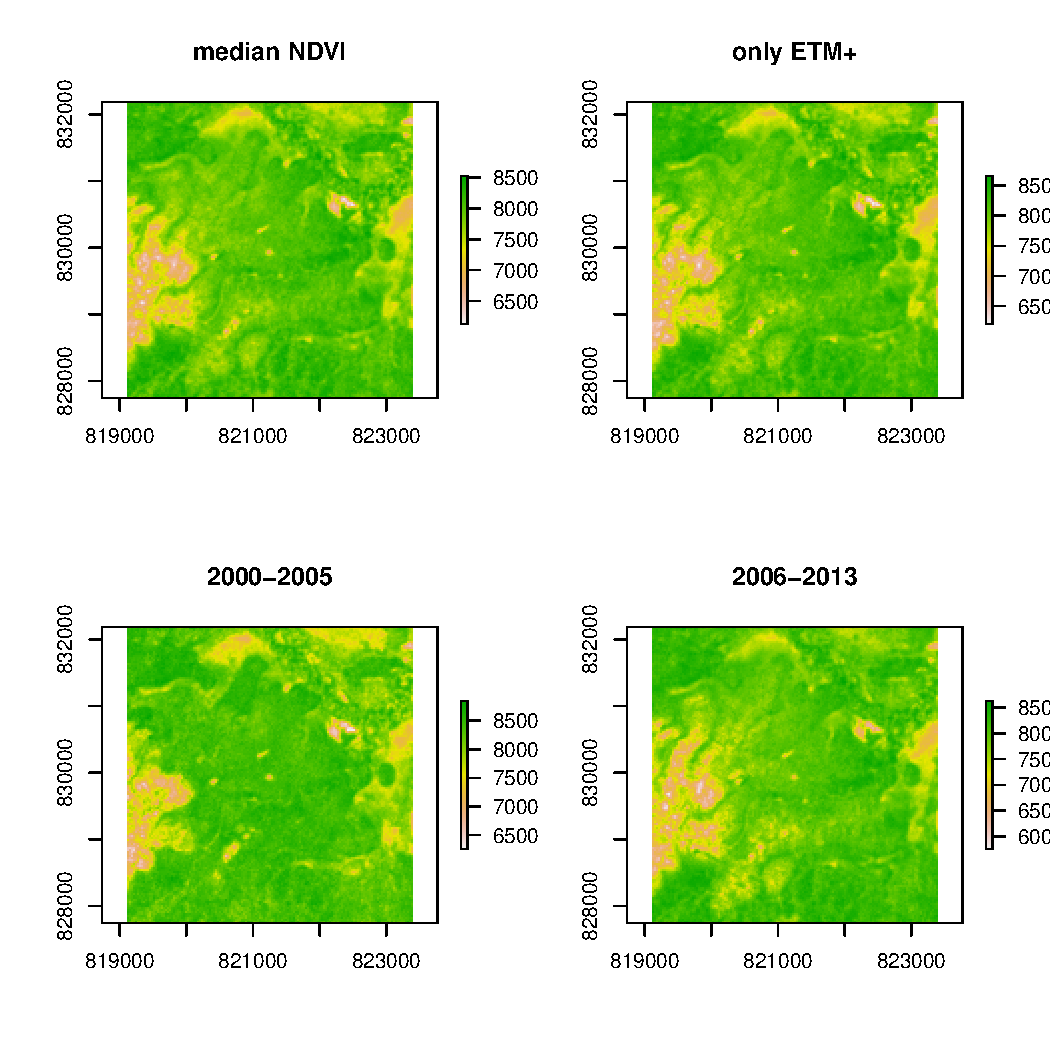
\includegraphics[width=\maxwidth]{figure/summaryBrick-dates} 
\begin{kframe}\begin{alltt}
\hlkwd{par}\hlstd{(op)}
\end{alltt}
\end{kframe}
\end{knitrout}


\code{minDate} and \code{maxDate} can be supplied in one of two ways: (1) as a character or date object in the format \code{"\%Y-\%m-\%d"} (eg. ``2013-01-31") or (2) as a numeric vector of length 2 representing the year and Julian day (e.g. \code{c(2013, 31)}).

Note that the Tura brick already has scene information included as layer names (see \code{names(tura)}). To run \code{annualSummary} on RasterBricks where no scene information is available, a dates vector \emph{must} be supplied to be able to divide the layers into years. This vector is also required for \code{summaryBrick} when constraining the calculation by date using \code{minDate} and \code{maxDate}.

\code{annualSummary} works similarly to \code{summaryBrick}, but provides a statistic for each year of the time series. At this time, this function is only applicable to Landsat data, and the scene IDs must be supplied either as \code{names(x)} or as a separate character vector to \code{sceneID}. In this sample, we will again calculate median NDVI on all ETM+ data, but this time we are interested in seeing the \emph{annual} median NDVI value.

\begin{knitrout}
\definecolor{shadecolor}{rgb}{0.969, 0.969, 0.969}\color{fgcolor}\begin{kframe}
\begin{alltt}
\hlstd{annualMed} \hlkwb{<-} \hlkwd{annualSummary}\hlstd{(tura,} \hlkwc{fun} \hlstd{= median,} \hlkwc{sensor} \hlstd{=} \hlstr{"ETM+"}\hlstd{,} \hlkwc{na.rm} \hlstd{=} \hlnum{TRUE}\hlstd{)}
\hlkwd{plot}\hlstd{(annualMed)}
\end{alltt}
\end{kframe}
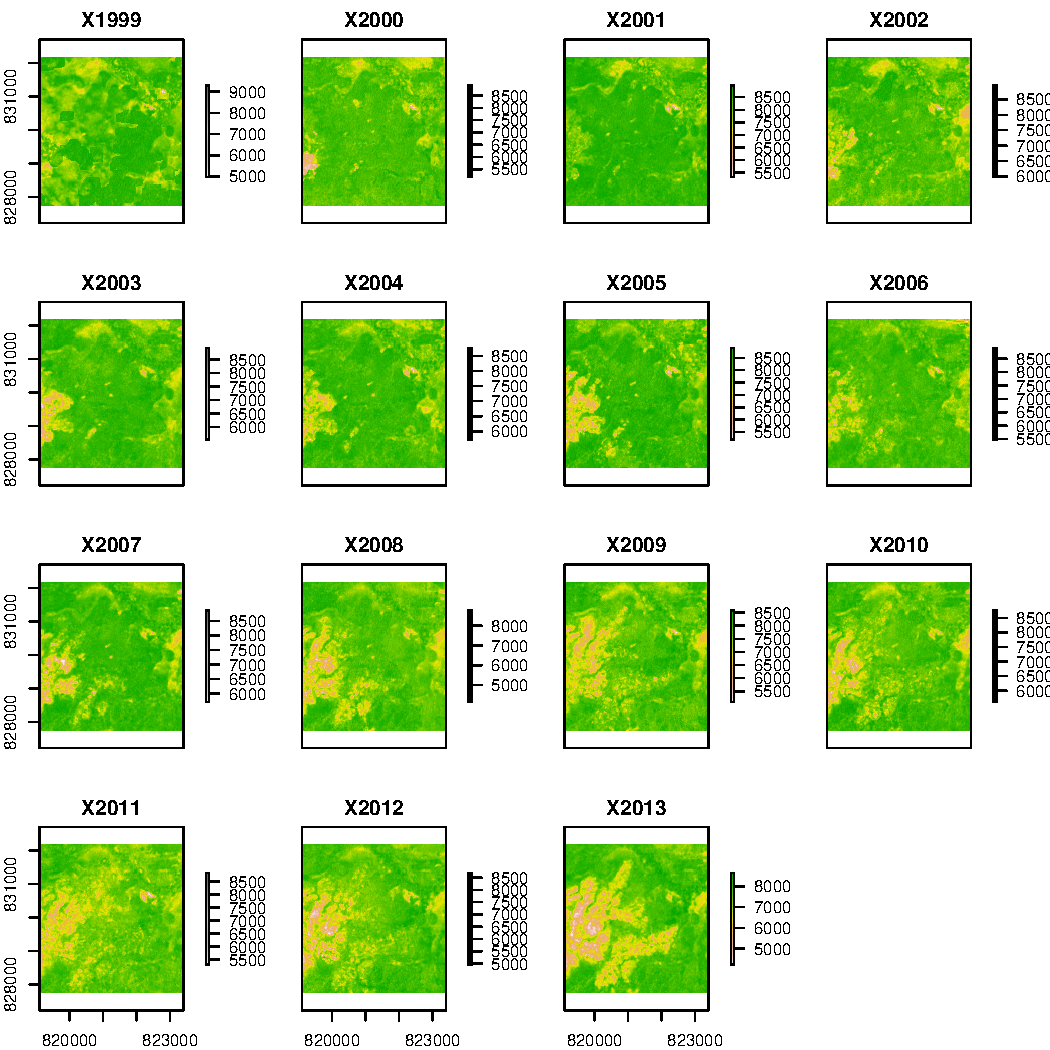
\includegraphics[width=\maxwidth]{figure/annualSummary-ETM} 

\end{knitrout}


Both \code{summaryBrick()} and \code{annualSummary()} can pass additional arguments to \code{mc.calc()}, meaning that the result can be saved to file with a \code{filename} argument, and multiple cores can be used in the calculation with a \code{mc.cores} argument.

From the summary RasterBrick above, we can see that this is a very dynamic area, with some of the biggest forest changes occurring from 2009 until 2013. With the help of \code{bfastmonitor}, we will look at ways to quantify and map these changes at high temporal resolution.

\section{Spatial BFASTMonitor}

\subsection{Working with pixels: \code{bfmPixel}}

Working with \code{bfastmonitor} (BFM) can be intimidating at first, especially given the number of parameters that need to be set (or at least considered) before running the algorithm. It is important to understand these parameters, as not all raster time series are equal. Some time series may have frequent and large temporal gaps (as can be expected in some tropical forest), while others are temporally dense. These differences may call for slightly different approaches in implementing BFM.

\code{bfmPixel} is a function which queries individual pixels in a raster time series and runs bfm over that pixel's time series. To run \code{bfmPixel} in interactive mode, one of the layers of the time series needs to first be plotted.

\begin{knitrout}
\definecolor{shadecolor}{rgb}{0.969, 0.969, 0.969}\color{fgcolor}\begin{kframe}
\begin{alltt}
\hlcom{# load tura RasterBrick}
\hlkwd{data}\hlstd{(tura)}
\hlcom{# plot the 6h layer}
\hlkwd{plot}\hlstd{(tura,} \hlnum{6}\hlstd{)}
\hlcom{# run bfmPixel() in interactive mode with a monitoring period starting @ the}
\hlcom{# 1st day in 2009}
\hlstd{bfm} \hlkwb{<-} \hlkwd{bfmPixel}\hlstd{(tura,} \hlkwc{start} \hlstd{=} \hlkwd{c}\hlstd{(}\hlnum{2009}\hlstd{,} \hlnum{1}\hlstd{),} \hlkwc{interactive} \hlstd{=} \hlnum{TRUE}\hlstd{)}
\end{alltt}
\end{kframe}
\end{knitrout}


Inspecting the output of this function, you will see that a list of length 2 has been outputted. First, a list of class \code{bfastmonitor} is output under \code{\$bfm}. Second, an integer indicating the cell number that has been clicked is output under \code{\$cell}. The output is formatted this way so that if \code{bfmPixel} is run in interactive mode, a follow-up analysis can be done on that same cell without having to guess which cell was clicked before. In the above example, the cell number can be retrieved simply by typing \code{bfm\$cell} in the console.

Let's run \code{bfmPixel} again, but this time indicating a specific cell number instead of using interactive mode. Note that by default \code{interactive=FALSE}, so there is no need to specify this if a value for \code{cell} is given.

\begin{knitrout}
\definecolor{shadecolor}{rgb}{0.969, 0.969, 0.969}\color{fgcolor}\begin{kframe}
\begin{alltt}
\hlstd{targcell} \hlkwb{<-} \hlnum{3492}
\hlstd{bfm} \hlkwb{<-} \hlkwd{bfmPixel}\hlstd{(tura,} \hlkwc{cell} \hlstd{= targcell,} \hlkwc{start} \hlstd{=} \hlkwd{c}\hlstd{(}\hlnum{2009}\hlstd{,} \hlnum{1}\hlstd{))}
\hlcom{# inspect and plot the $bfm output}
\hlstd{bfm}\hlopt{$}\hlstd{bfm}
\end{alltt}
\begin{verbatim}
## 
## BFAST monitoring
## 
## 1. History period
## Stable period selected: 1984(285)--2008(359)
## Length (in years): 24.202740
## Model fit:
## (Intercept)       trend  harmoncos1  harmoncos2  harmoncos3  harmonsin1 
##  7577.91041     0.09905  -297.47432    71.66341    52.05172  -393.96794 
##  harmonsin2  harmonsin3 
##     5.38914   -36.69532 
## R-squared: 0.360894
## 
## 
## 2. Monitoring period
## Monitoring period assessed: 2009(1)--2013(101)
## Length (in years): 4.273973
## Break detected at: 2009(298)
\end{verbatim}
\begin{alltt}
\hlkwd{plot}\hlstd{(bfm}\hlopt{$}\hlstd{bfm)}
\end{alltt}
\end{kframe}
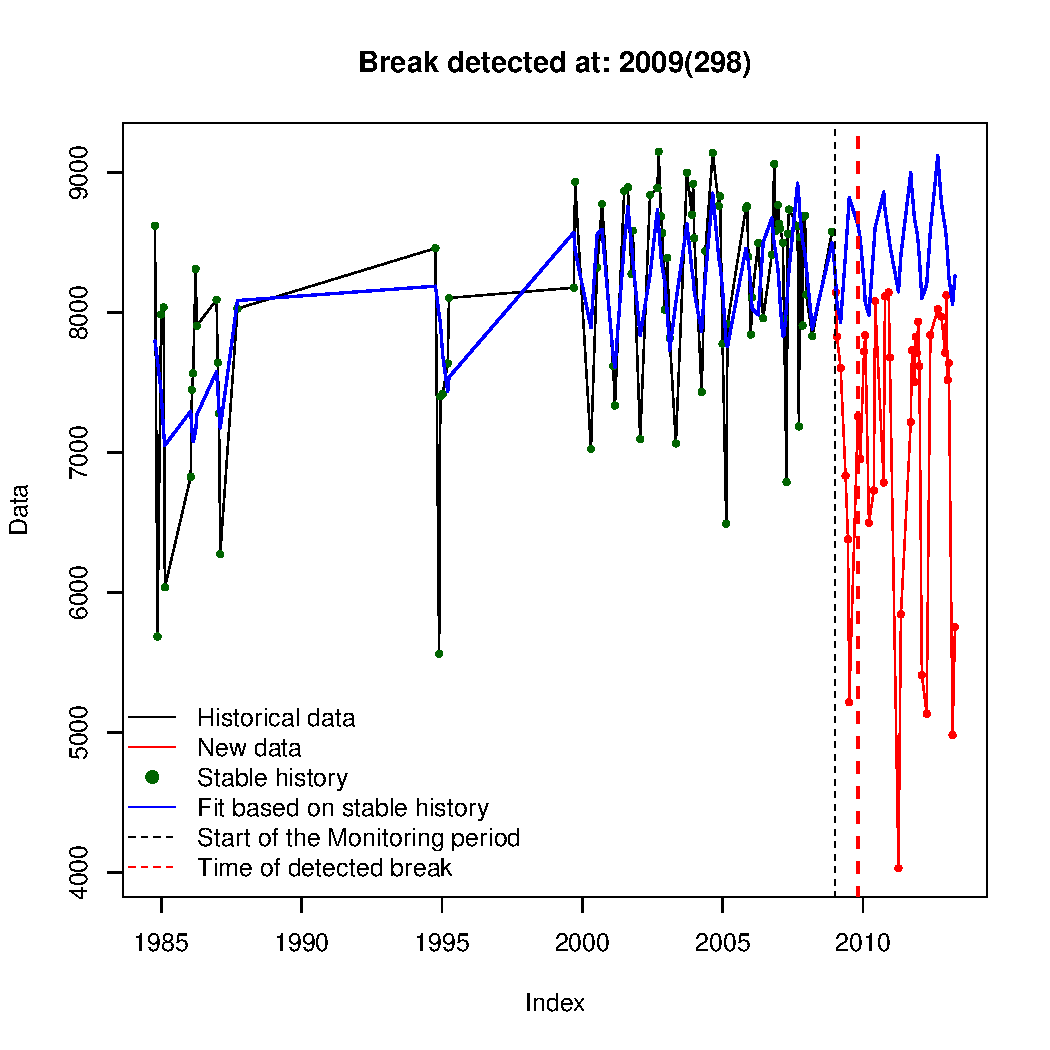
\includegraphics[width=\maxwidth]{figure/bfmPixel-targcell} 

\end{knitrout}


Specifying a cell number gives the advantage of being able to test different parameters on the same pixel time series to see what impact these parameters have on the sensitivity of the algorithm. Note that a plot is immediately produced if \code{plot = TRUE}.

\begin{knitrout}
\definecolor{shadecolor}{rgb}{0.969, 0.969, 0.969}\color{fgcolor}\begin{kframe}
\begin{alltt}
\hlcom{# use a harmonic model only}
\hlstd{bfm1} \hlkwb{<-} \hlkwd{bfmPixel}\hlstd{(tura,} \hlkwc{cell} \hlstd{= targcell,} \hlkwc{start} \hlstd{=} \hlkwd{c}\hlstd{(}\hlnum{2009}\hlstd{,} \hlnum{1}\hlstd{),} \hlkwc{formula} \hlstd{= response} \hlopt{~}
    \hlstd{harmon,} \hlkwc{plot} \hlstd{=} \hlnum{TRUE}\hlstd{)}
\end{alltt}
\end{kframe}
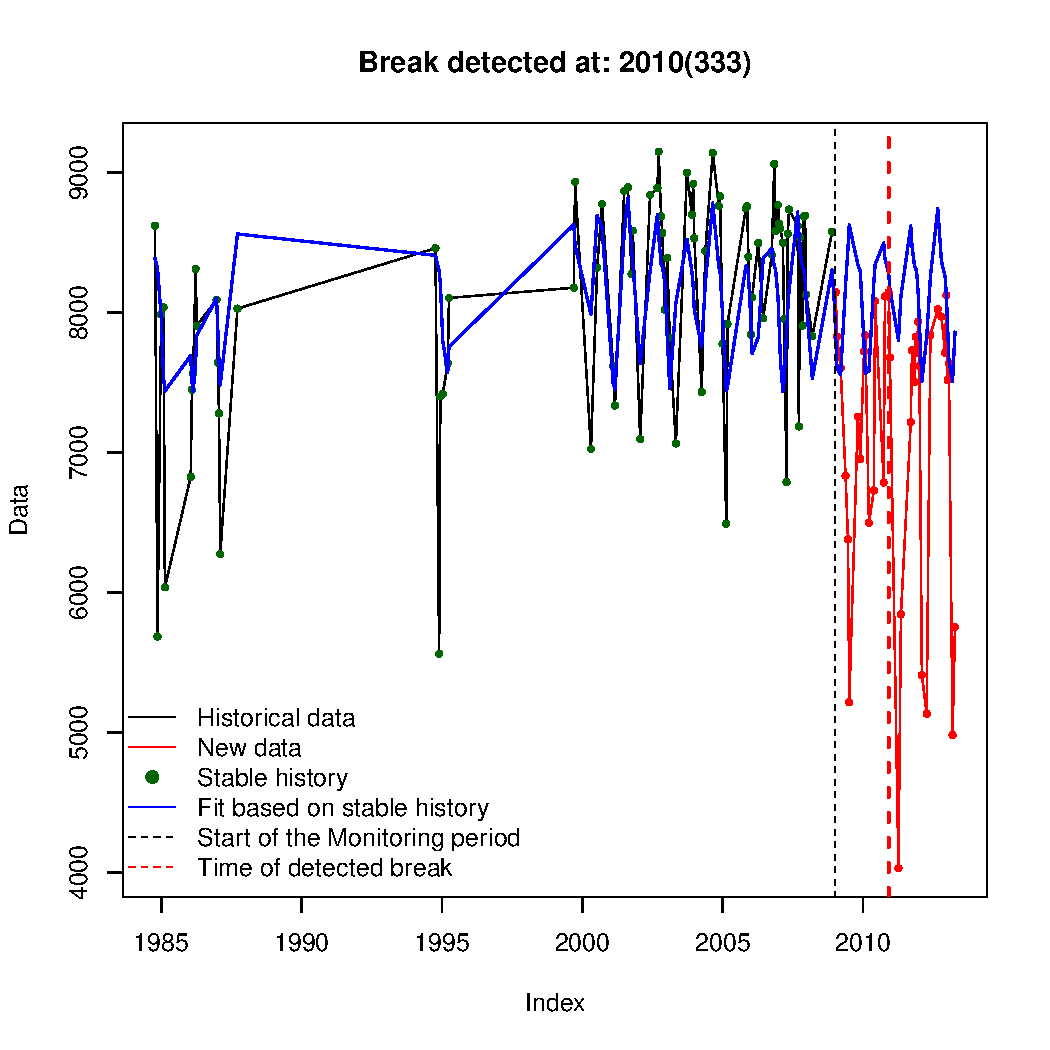
\includegraphics[width=\maxwidth]{figure/bfmPixel-args1} 
\begin{kframe}\begin{alltt}
\hlcom{# same, but with an order of 1}
\hlstd{bfm2} \hlkwb{<-} \hlkwd{bfmPixel}\hlstd{(tura,} \hlkwc{cell} \hlstd{= targcell,} \hlkwc{start} \hlstd{=} \hlkwd{c}\hlstd{(}\hlnum{2009}\hlstd{,} \hlnum{1}\hlstd{),} \hlkwc{formula} \hlstd{= response} \hlopt{~}
    \hlstd{harmon,} \hlkwc{order} \hlstd{=} \hlnum{1}\hlstd{,} \hlkwc{plot} \hlstd{=} \hlnum{TRUE}\hlstd{)}
\end{alltt}
\end{kframe}
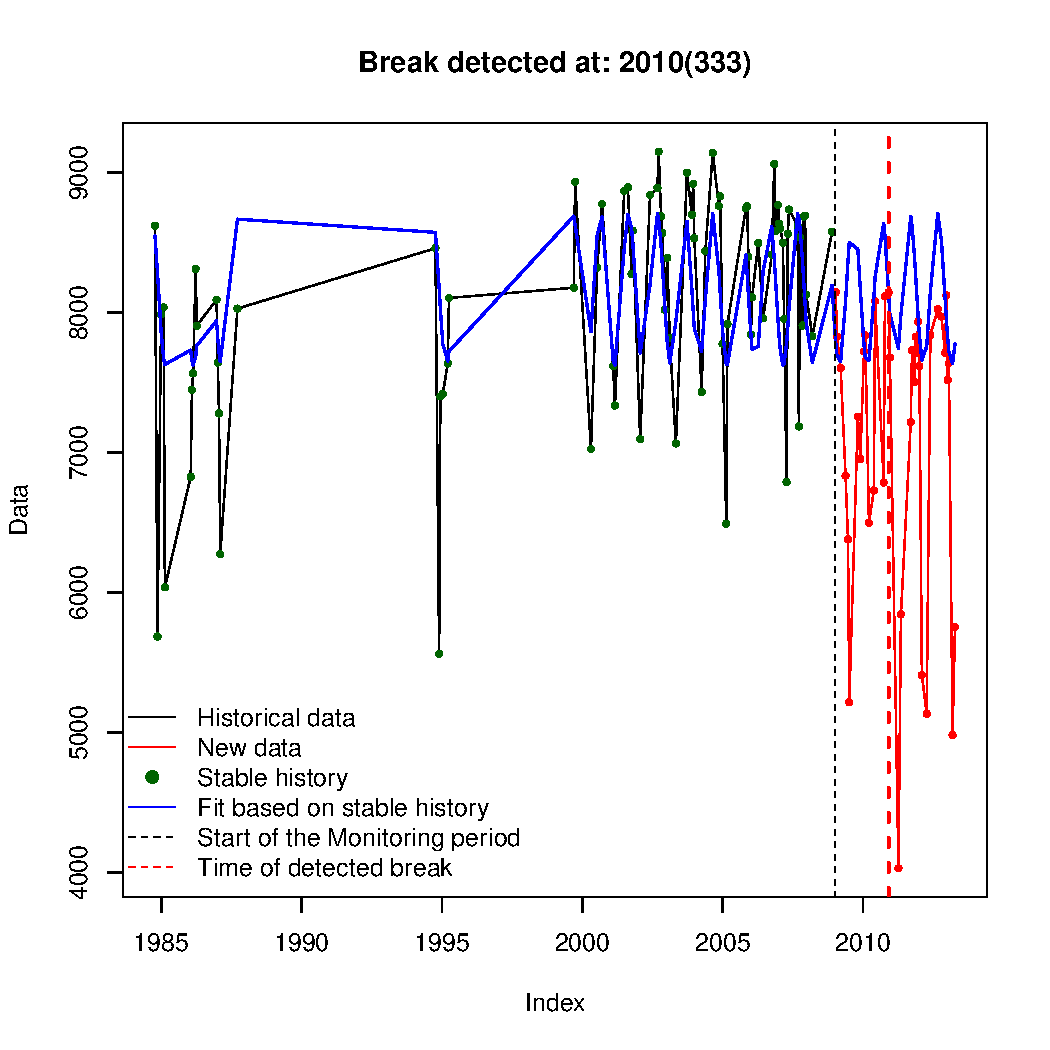
\includegraphics[width=\maxwidth]{figure/bfmPixel-args2} 
\begin{kframe}\begin{alltt}
\hlcom{# only trend}
\hlstd{bfm3} \hlkwb{<-} \hlkwd{bfmPixel}\hlstd{(tura,} \hlkwc{cell} \hlstd{= targcell,} \hlkwc{start} \hlstd{=} \hlkwd{c}\hlstd{(}\hlnum{2009}\hlstd{,} \hlnum{1}\hlstd{),} \hlkwc{formula} \hlstd{= response} \hlopt{~}
    \hlstd{trend,} \hlkwc{plot} \hlstd{=} \hlnum{TRUE}\hlstd{)}
\end{alltt}
\end{kframe}
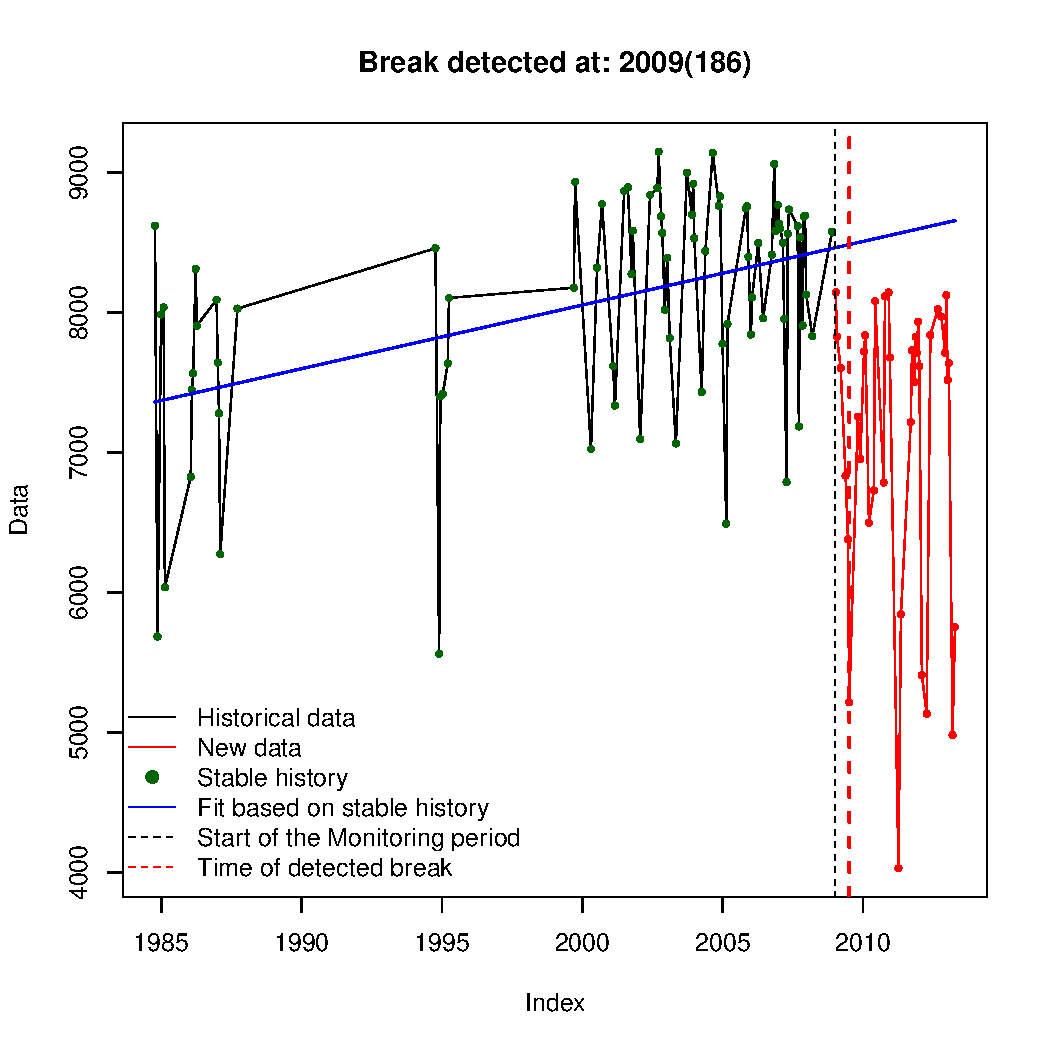
\includegraphics[width=\maxwidth]{figure/bfmPixel-args3} 

\end{knitrout}


Check out \code{?bfastmonitor} for more information on the parameters that are included in the method.

A number of additional options are provided in \code{bfmPixel}. Specifying a value for \code{monend} will trim the time series after that date (thus limiting the monitoring period to a given period). This simple modification can have an impact on the resulting change magnitude, which is computed as the median residual between the predicted and observed values within the monitoring period.

\begin{knitrout}
\definecolor{shadecolor}{rgb}{0.969, 0.969, 0.969}\color{fgcolor}\begin{kframe}
\begin{alltt}
\hlcom{# bfmPixel using a 1-year monitoring period}
\hlstd{bfm4} \hlkwb{<-} \hlkwd{bfmPixel}\hlstd{(tura,} \hlkwc{cell} \hlstd{= targcell,} \hlkwc{start} \hlstd{=} \hlkwd{c}\hlstd{(}\hlnum{2009}\hlstd{,} \hlnum{1}\hlstd{),} \hlkwc{monend} \hlstd{=} \hlkwd{c}\hlstd{(}\hlnum{2010}\hlstd{,}
    \hlnum{1}\hlstd{),} \hlkwc{plot} \hlstd{=} \hlnum{TRUE}\hlstd{)}
\end{alltt}
\end{kframe}
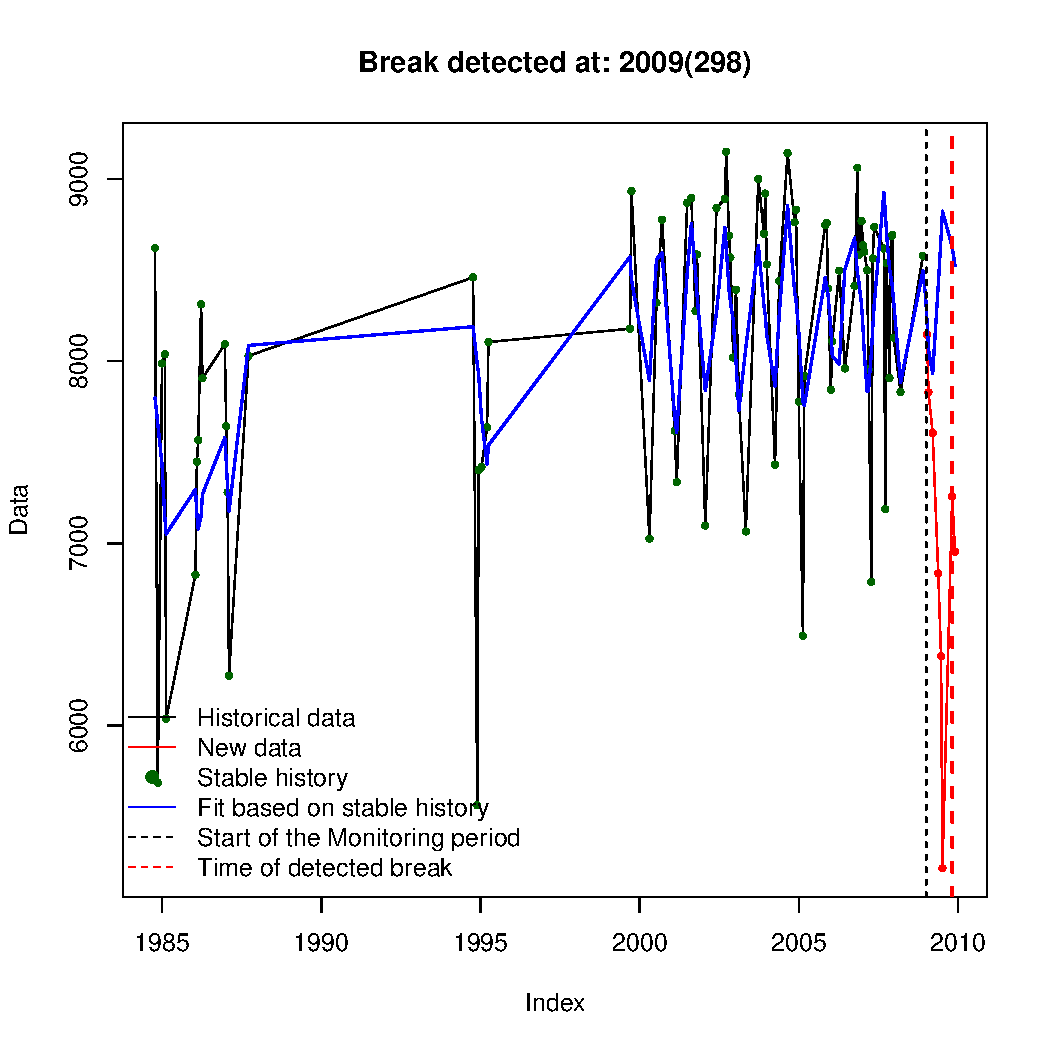
\includegraphics[width=\maxwidth]{figure/bfmPixel-monend} 

\end{knitrout}


Finally, for Landsat time series the analysis can be limited to data of a specific sensor. The \code{sensor} parameter currently accepts the following possible character values:
\begin{itemize}
\item \code{"ETM+"}
\item \code{"ETM+ SLC-on"}
\item \code{"ETM+ SLC-off"}
\item \code{"TM"}
\end{itemize}

Note that in our previous runs of \code{bfmPixel}, there is what seems to be a bias between TM data from the 80's and 90's (which can be found throughout the scene). This has a large effect on our model, especially when a trend is included. A very quick way to avoid this bias is to include only data from the ETM+ sensor, which was launched in 1999.

\begin{knitrout}
\definecolor{shadecolor}{rgb}{0.969, 0.969, 0.969}\color{fgcolor}\begin{kframe}
\begin{alltt}
\hlcom{# apply bfmPixel only on ETM+ data}
\hlstd{bfm5} \hlkwb{<-} \hlkwd{bfmPixel}\hlstd{(tura,} \hlkwc{cell} \hlstd{= targcell,} \hlkwc{start} \hlstd{=} \hlkwd{c}\hlstd{(}\hlnum{2009}\hlstd{,} \hlnum{1}\hlstd{),} \hlkwc{sensor} \hlstd{=} \hlstr{"ETM+"}\hlstd{,}
    \hlkwc{plot} \hlstd{=} \hlnum{TRUE}\hlstd{)}
\end{alltt}
\end{kframe}
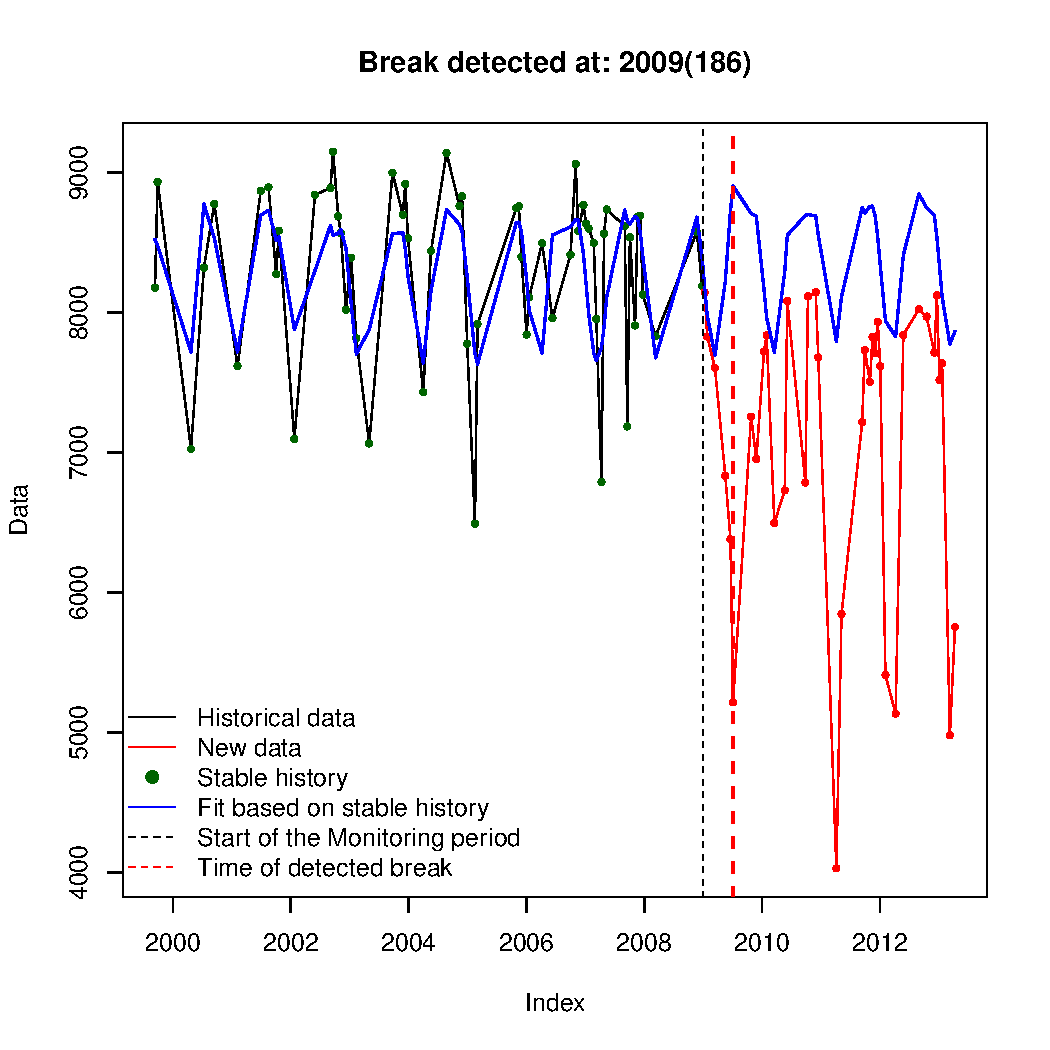
\includegraphics[width=\maxwidth]{figure/bfmPixel-sensor} 

\end{knitrout}


\subsection{Working with raster time series: \code{bfmSpatial}}

Now that we have done some pixel-based testing, it is time to apply \code{bfastmonitor} over an entire raster time series. This will allow us to pinpoint the location and timing of changes in our study area. In the previous section, we saw that there was a large gap in the 1990's in the tura raster time series, and given the acceptable data density, we could just limit the analysis to ETM+ data. We also saw that a harmonic-trend model with an order of 1 seemed to be the most reasonable time series model for the tura dataset. We will pass these same arguments to \code{bfmSpatial}. At the same time, we will calculate how long the process takes by wrapping it in a \code{system.time} call.




\begin{knitrout}
\definecolor{shadecolor}{rgb}{0.969, 0.969, 0.969}\color{fgcolor}\begin{kframe}
\begin{alltt}
\hlcom{# run bfmSpatial over tura for a monitoring period of 2009 -}
\hlstd{t1} \hlkwb{<-} \hlkwd{system.time}\hlstd{(bfm} \hlkwb{<-} \hlkwd{bfmSpatial}\hlstd{(tura,} \hlkwc{start} \hlstd{=} \hlkwd{c}\hlstd{(}\hlnum{2009}\hlstd{,} \hlnum{1}\hlstd{),} \hlkwc{order} \hlstd{=} \hlnum{1}\hlstd{))}
\hlcom{# plot the result}
\hlkwd{plot}\hlstd{(bfm)}
\end{alltt}
\end{kframe}
\end{knitrout}


Luckily for us, tura is a very small RasterBrick, and processing is not incredibly time consuming. Realistically, analyses are done over significantly larger areas (possibly extending beyond a single scene), so running \code{bfmSpatial} on such large areas quickly becomes a very time-consuming task. To assist in this, multi-core support has been built into \code{bfmSpatial}, using the \code{parallel} package. Let's run the same line of code again, but this time specify a value for \code{mc.cores}, which will distribute the process over that many cpus. Again, we will wrap the code in a \code{system.time} call to test the speed of the processing.

\begin{knitrout}
\definecolor{shadecolor}{rgb}{0.969, 0.969, 0.969}\color{fgcolor}\begin{kframe}
\begin{alltt}
\hlstd{t2} \hlkwb{<-} \hlkwd{system.time}\hlstd{(bfm} \hlkwb{<-} \hlkwd{bfmSpatial}\hlstd{(tura,} \hlkwc{start} \hlstd{=} \hlkwd{c}\hlstd{(}\hlnum{2009}\hlstd{,} \hlnum{1}\hlstd{),} \hlkwc{order} \hlstd{=} \hlnum{1}\hlstd{,} \hlkwc{mc.cores} \hlstd{=} \hlnum{8}\hlstd{))}
\hlcom{# compare processing time with previous run}
\hlstd{t1} \hlopt{-} \hlstd{t2}
\end{alltt}
\end{kframe}
\end{knitrout}


%% option: include something from parallel package regarding checking # of available cores, etc...?
%% or something like 'good practices in parallel computing'? Or could that be covered in the pre-processing module?

\section{Post-Processing of BFM output}

Three raster layers are output by \code{bfmSpatial}:
\begin{enumerate}
\item breakpoint timing - in decimal year format
\item change magnitude - the medial residual between expected and observed values in the monitoring period
\item error flag - possible values of 1 if an error has been encountered in a particular pixel, and NA where the algorithm was successful (or a mask had already been applied previously)
\end{enumerate}

The \code{bfastSpatial} package has some simple functions for 'unpacking' the \code{bfmSpatial} results. \code{bfmChange} simply extracts the first layer and saves it to a separate object.

\begin{knitrout}
\definecolor{shadecolor}{rgb}{0.969, 0.969, 0.969}\color{fgcolor}\begin{kframe}
\begin{alltt}
\hlcom{# extract change raster}
\hlstd{change} \hlkwb{<-} \hlkwd{bfmChange}\hlstd{(bfm)}
\end{alltt}
\end{kframe}
\end{knitrout}


The change raster gives breakpoint timing values in decimal years. A better way to map change timing from these results may be to show the month of change (the validity of this depends on the temporal density of there input time series). \code{changeMonth} is a convenient way to convert breakpoint values to change months. The result is one or more raster layers with integer values between 1 and 12, representing the months of the year. In cases where multiple years are represented in the change raster, these are split into raster layers representing one layer per year.

\begin{knitrout}
\definecolor{shadecolor}{rgb}{0.969, 0.969, 0.969}\color{fgcolor}\begin{kframe}
\begin{alltt}
\hlstd{months} \hlkwb{<-} \hlkwd{changeMonth}\hlstd{(change)}
\hlcom{# set up labels and colourmap for months}
\hlstd{monthlabs} \hlkwb{<-} \hlkwd{c}\hlstd{(}\hlstr{"jan"}\hlstd{,} \hlstr{"feb"}\hlstd{,} \hlstr{"mar"}\hlstd{,} \hlstr{"apr"}\hlstd{,} \hlstr{"may"}\hlstd{,} \hlstr{"jun"}\hlstd{,} \hlstr{"jul"}\hlstd{,} \hlstr{"aug"}\hlstd{,} \hlstr{"sep"}\hlstd{,}
    \hlstr{"oct"}\hlstd{,} \hlstr{"nov"}\hlstd{,} \hlstr{"dec"}\hlstd{)}
\hlkwd{library}\hlstd{(RColorBrewer)}
\hlstd{cols} \hlkwb{<-} \hlkwd{rev}\hlstd{(}\hlkwd{brewer.pal}\hlstd{(}\hlnum{11}\hlstd{,} \hlstr{"RdYlBu"}\hlstd{))}
\hlcom{# interpolate colormap (since max # of colours for 'RdYlBu' is 11)}
\hlstd{cols} \hlkwb{<-} \hlkwd{colorRampPalette}\hlstd{(cols)(}\hlnum{12}\hlstd{)}
\hlkwd{plot}\hlstd{(months,} \hlkwc{col} \hlstd{= cols,} \hlkwc{breaks} \hlstd{=} \hlkwd{c}\hlstd{(}\hlnum{1}\hlopt{:}\hlnum{12}\hlstd{),} \hlkwc{legend} \hlstd{=} \hlnum{FALSE}\hlstd{)}
\hlcom{# insert custom legend}
\hlkwd{legend}\hlstd{(}\hlstr{"bottomright"}\hlstd{,} \hlkwc{legend} \hlstd{= monthlabs,} \hlkwc{cex} \hlstd{=} \hlnum{0.5}\hlstd{,} \hlkwc{fill} \hlstd{= cols,} \hlkwc{ncol} \hlstd{=} \hlnum{2}\hlstd{)}
\end{alltt}
\end{kframe}
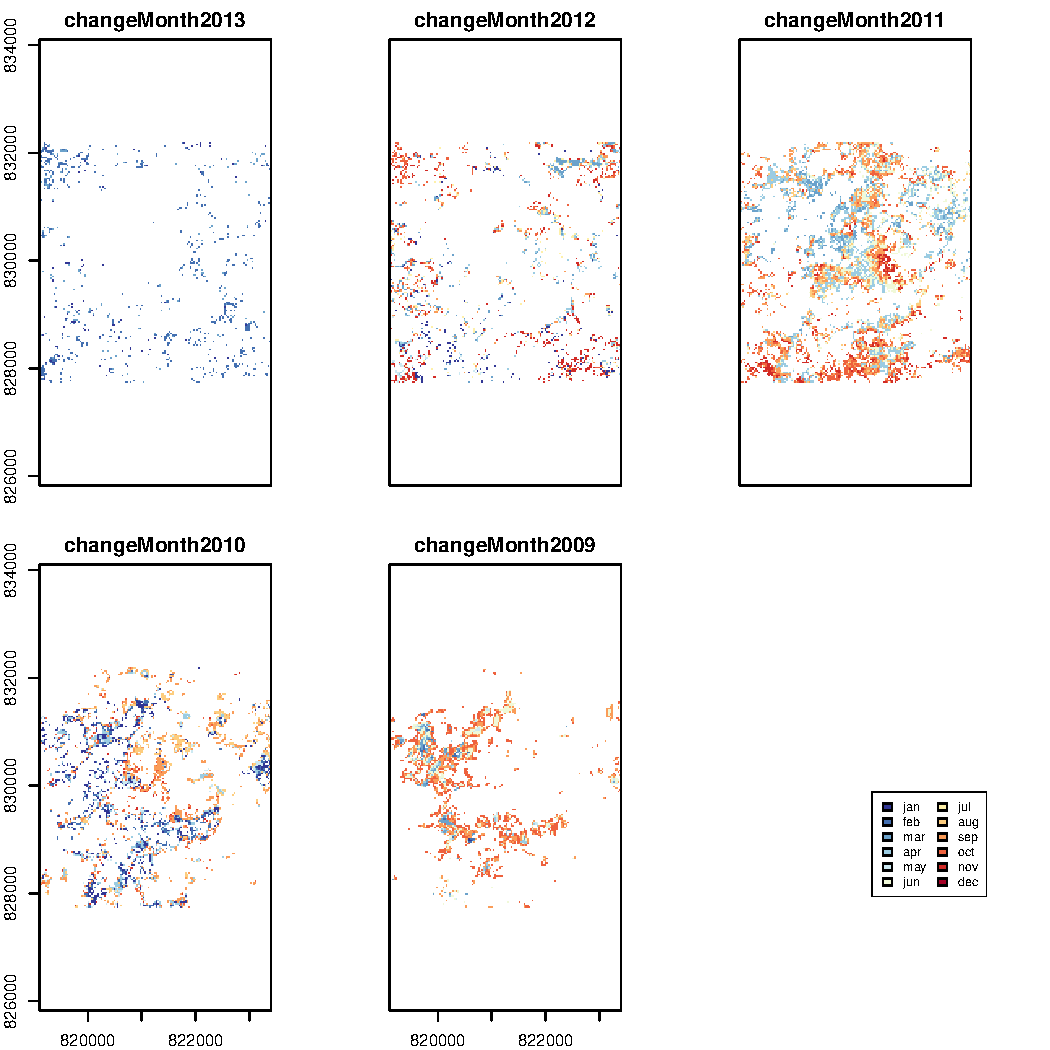
\includegraphics[width=\maxwidth]{figure/changeMonth} 

\end{knitrout}


\code{bfmMagn} does the same as \code{bfmChange} to the second layer, but adds some other options (masking by breakpoint, applying a threshold). Magnitude is computed as the median residual between expected and observed values throughout the \emph{entire} monitoring period, meaning that all pixels are assigned a value regardless of whether or not a breakpoint has been detected. If we are only interested in looking at pixels where a breakpoint has been detected, we can use the \code{change} argument in the \code{bfmMagn}, which takes a raster of breakpoints to use as a filter.

\begin{knitrout}
\definecolor{shadecolor}{rgb}{0.969, 0.969, 0.969}\color{fgcolor}\begin{kframe}
\begin{alltt}
\hlcom{# extract magn raster, and include only change pixels}
\hlstd{magn} \hlkwb{<-} \hlkwd{bfmMagn}\hlstd{(bfm,} \hlkwc{change} \hlstd{= change)}
\hlcom{# compare with 'original' magn raster}
\hlstd{op} \hlkwb{<-} \hlkwd{par}\hlstd{(}\hlkwc{mfrow} \hlstd{=} \hlkwd{c}\hlstd{(}\hlnum{1}\hlstd{,} \hlnum{2}\hlstd{))}
\hlkwd{plot}\hlstd{(magn,} \hlkwc{main} \hlstd{=} \hlstr{"Magnitude: breakpoints"}\hlstd{)}
\hlkwd{plot}\hlstd{(bfm[[}\hlnum{2}\hlstd{]],} \hlkwc{main} \hlstd{=} \hlstr{"Magnitude: all pixels"}\hlstd{)}
\end{alltt}
\end{kframe}
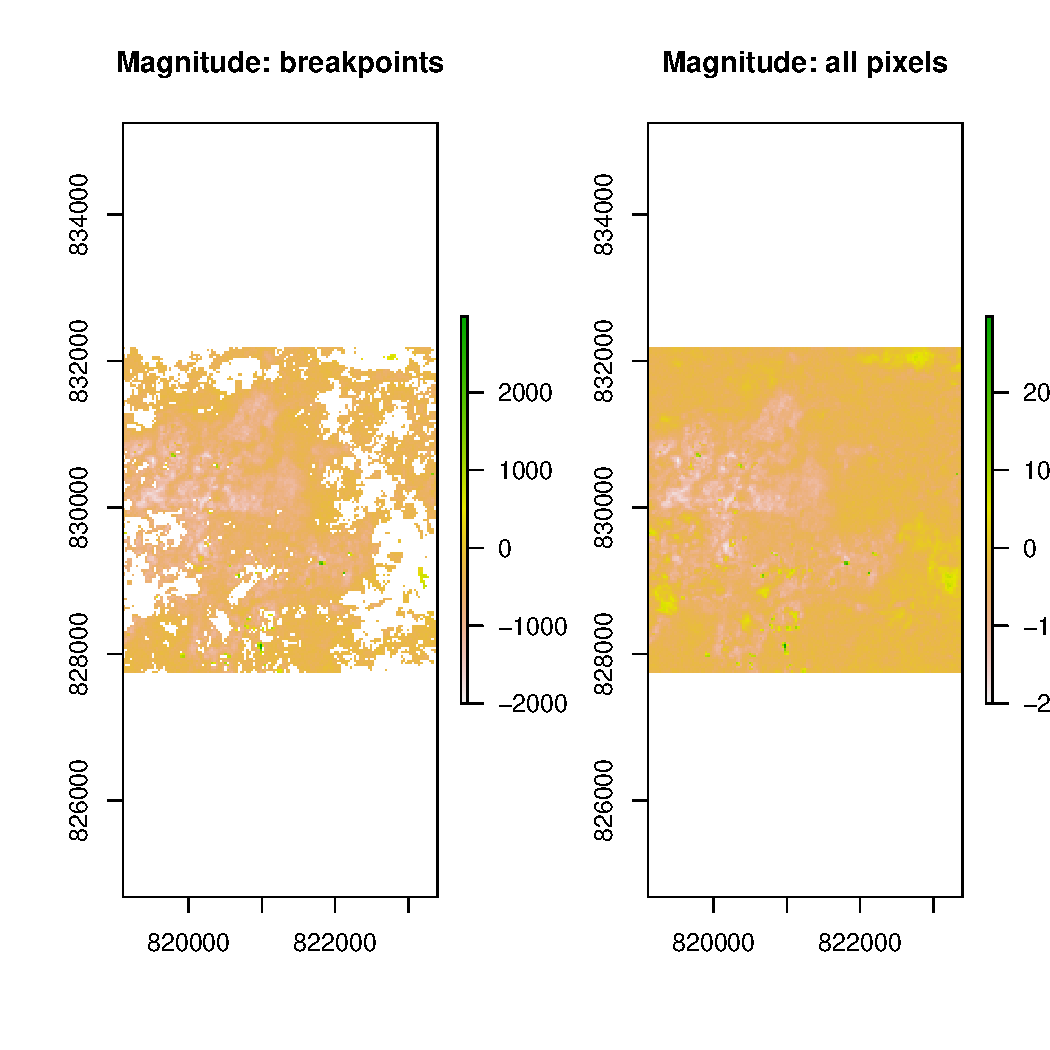
\includegraphics[width=\maxwidth]{figure/bfmMagn} 
\begin{kframe}\begin{alltt}
\hlkwd{par}\hlstd{(op)}
\end{alltt}
\end{kframe}
\end{knitrout}


Note that the magnitude values are in the same scale as the input data, which had been scaled by 10000. Scaling back can be done by simple raster algebra, or with the \code{raster::calc} function to enable writing to file.

\begin{knitrout}
\definecolor{shadecolor}{rgb}{0.969, 0.969, 0.969}\color{fgcolor}\begin{kframe}
\begin{alltt}
\hlstd{magn} \hlkwb{<-} \hlkwd{bfmMagn}\hlstd{(bfm,} \hlkwc{change} \hlstd{= change)}\hlopt{/}\hlnum{10000}
\end{alltt}
\end{kframe}
\end{knitrout}


The magnitude could be used to discriminate between actual deforestation and other factors that might give rise to breakpoints (such as noisy data). However, interpreting magnitude is complicated by the fact that follow-up dynamics can affect the magnitude value, since it is computed throughout the entire monitoring period. To circumvent this (not entirely), we will re-run \code{bfmSpatial} using a 1-year monitoring period, under the assumption that this monitoring window is too short for post-change dynamics to significantly affect the magnitude value. To do this, we will include the \code{monend} argument of \code{bfmSpatial}, which will limit the analysis to a specific time period. In this example, we will use a 2009-2010 monitoring period with all other parameters the same as above.




\begin{knitrout}
\definecolor{shadecolor}{rgb}{0.969, 0.969, 0.969}\color{fgcolor}\begin{kframe}
\begin{alltt}
\hlstd{bfm09} \hlkwb{<-} \hlkwd{bfmSpatial}\hlstd{(tura,} \hlkwc{start} \hlstd{=} \hlkwd{c}\hlstd{(}\hlnum{2009}\hlstd{,} \hlnum{1}\hlstd{),} \hlkwc{monend} \hlstd{=} \hlkwd{c}\hlstd{(}\hlnum{2010}\hlstd{,} \hlnum{1}\hlstd{),} \hlkwc{order} \hlstd{=} \hlnum{1}\hlstd{)}
\hlcom{# extract change}
\hlstd{change09} \hlkwb{<-} \hlkwd{bfmChange}\hlstd{(bfm09)}
\hlcom{# extract and rescale magnitude}
\hlstd{magn09} \hlkwb{<-} \hlkwd{bfmMagn}\hlstd{(bfm09,} \hlkwc{change} \hlstd{= change09)}\hlopt{/}\hlnum{10000}
\end{alltt}
\end{kframe}
\end{knitrout}


Suppose we know from field observations or other reference data that breakpoints with NDVI magnitudes of -0.05 are associated with high probability of detected actual deforestation. We can easily apply this threshold to our magnitude raster, or even pass this threshold as an additional argument to \code{bfmMagn}. In the later case, take care with the scaling of the data - the original \code{bfmSpatial} results are still in their ``raw" format. In this case, our threshold should be accordingly scaled. In this example, we will scale the final magnitude back, as above.

\begin{knitrout}
\definecolor{shadecolor}{rgb}{0.969, 0.969, 0.969}\color{fgcolor}\begin{kframe}
\begin{alltt}
\hlcom{# extract and rescale magnitude and apply a -500 threshold}
\hlstd{magn09thresh} \hlkwb{<-} \hlkwd{bfmMagn}\hlstd{(bfm09,} \hlkwc{change} \hlstd{= change09,} \hlkwc{thresh} \hlstd{=} \hlopt{-}\hlnum{500}\hlstd{)}\hlopt{/}\hlnum{10000}
\hlcom{# compare}
\hlstd{op} \hlkwb{<-} \hlkwd{par}\hlstd{(}\hlkwc{mfrow} \hlstd{=} \hlkwd{c}\hlstd{(}\hlnum{1}\hlstd{,} \hlnum{2}\hlstd{))}
\hlkwd{plot}\hlstd{(magn09,} \hlkwc{main} \hlstd{=} \hlstr{"magnitude"}\hlstd{)}
\hlkwd{plot}\hlstd{(magn09thresh,} \hlkwc{main} \hlstd{=} \hlstr{"magnitude < -0.05"}\hlstd{)}
\end{alltt}
\end{kframe}
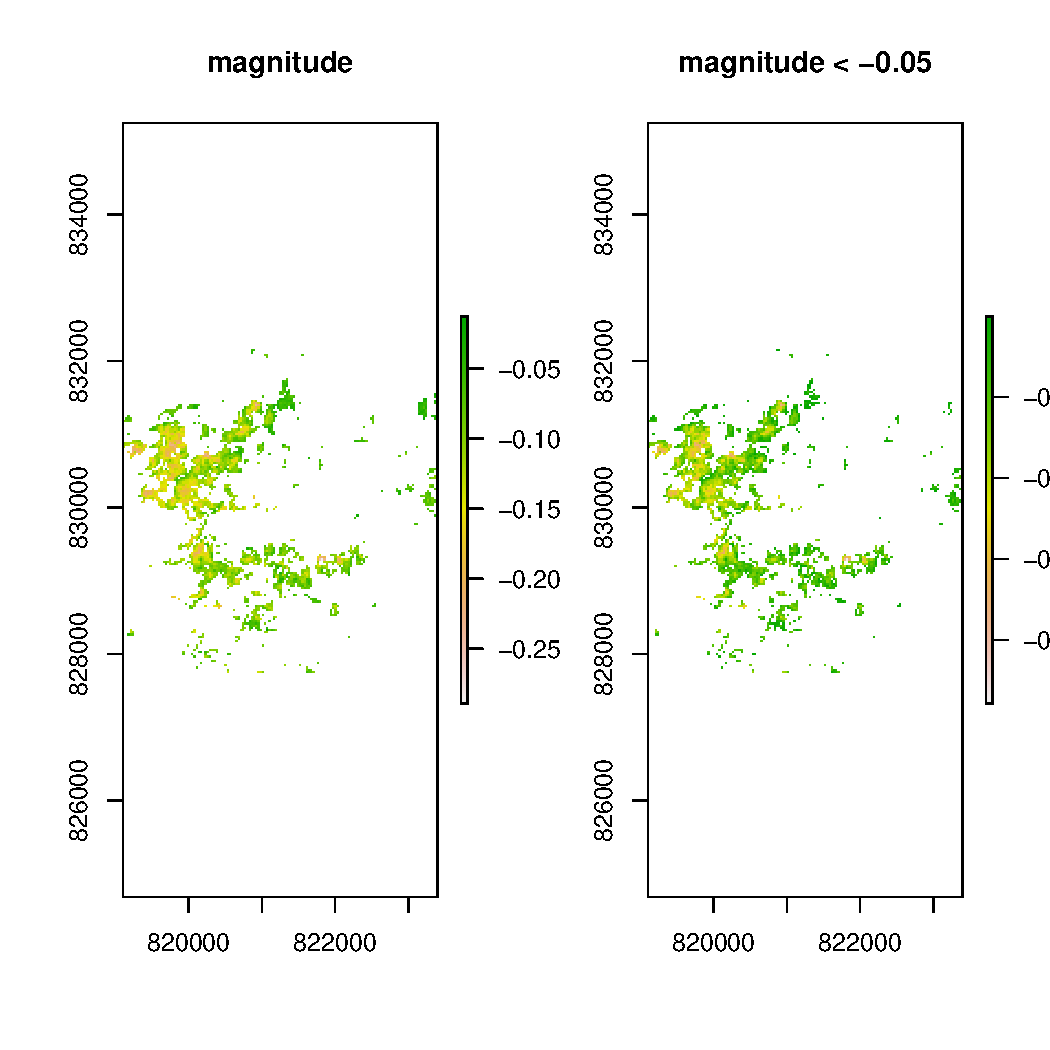
\includegraphics[width=\maxwidth]{figure/bfmMagn-thresh} 
\begin{kframe}\begin{alltt}
\hlkwd{par}\hlstd{(op)}
\end{alltt}
\end{kframe}
\end{knitrout}


A careful inspection of these results will show that applying the magnitude filter has changed the results somewhat, but since there isn't a great deal of noise in this example, the results were not dramatic. Another way we can clean up our results is to get rid of tiny clumps of change pixels that are not likely to represent actual change. For example, a simple raster sieve can eliminate single-pixel change clumps, which is justifiable given the fact that a Landsat pixel represents 900$m^2$, and detectable forest changes are expected to occur at larger scales. Note that the threshold has to be set on a ``less-than" basis, so we can use the area of 2 pixels as our cut-off.

\begin{knitrout}
\definecolor{shadecolor}{rgb}{0.969, 0.969, 0.969}\color{fgcolor}\begin{kframe}
\begin{alltt}
\hlstd{magn09_sieve} \hlkwb{<-} \hlkwd{areaSieve}\hlstd{(magn09thresh,} \hlkwc{thresh} \hlstd{=} \hlnum{1800}\hlstd{)}
\end{alltt}


{\ttfamily\noindent\itshape\color{messagecolor}{\#\# Loading required package: igraph}}\end{kframe}
\end{knitrout}


With \code{areaSieve}, this can be taken a step further, and an area threshold can be supplied to apply to the raster. \code{areaSieve} only supports thresholds in $m^2$, so be sure to do the appopriate conversions before appling the sieve. The default value is 5000, which corresponds to the 0.5ha forest definition often applied in national assessments.

\begin{knitrout}
\definecolor{shadecolor}{rgb}{0.969, 0.969, 0.969}\color{fgcolor}\begin{kframe}
\begin{alltt}
\hlstd{magn09_areasieve} \hlkwb{<-} \hlkwd{areaSieve}\hlstd{(magn09thresh)}  \hlcom{# default thresh = 5000}
\end{alltt}
\end{kframe}
\end{knitrout}


\code{areaSieve} passes additional arguments to \code{raster::clump}, which allows for considerations of direction when defining pixel neighbourhoods. \code{clump} adheres to the principle of ``queen's case" versus ``rook's case". In the former, pixels in all directions (default: \code{directions = 8}) are considered when defining clumps, whereas in the latter case, only pixels directly adjacent (excluding diagonals) are considered (\code{directions = 4}).

\begin{knitrout}
\definecolor{shadecolor}{rgb}{0.969, 0.969, 0.969}\color{fgcolor}\begin{kframe}
\begin{alltt}
\hlstd{magn09_as_rook} \hlkwb{<-} \hlkwd{areaSieve}\hlstd{(magn09thresh,} \hlkwc{directions} \hlstd{=} \hlnum{4}\hlstd{)}
\hlcom{# compare all magn rasters}
\hlstd{op} \hlkwb{<-} \hlkwd{par}\hlstd{(}\hlkwc{mfrow} \hlstd{=} \hlkwd{c}\hlstd{(}\hlnum{2}\hlstd{,} \hlnum{2}\hlstd{))}
\hlkwd{plot}\hlstd{(magn09thresh,} \hlkwc{main} \hlstd{=} \hlstr{"magnitude"}\hlstd{)}
\hlkwd{plot}\hlstd{(magn09_sieve,} \hlkwc{main} \hlstd{=} \hlstr{"pixel sieve"}\hlstd{)}
\hlkwd{plot}\hlstd{(magn09_areasieve,} \hlkwc{main} \hlstd{=} \hlstr{"0.5ha sieve"}\hlstd{)}
\hlkwd{plot}\hlstd{(magn09_as_rook,} \hlkwc{main} \hlstd{=} \hlstr{"0.5ha sieve, rook's case"}\hlstd{)}
\end{alltt}
\end{kframe}
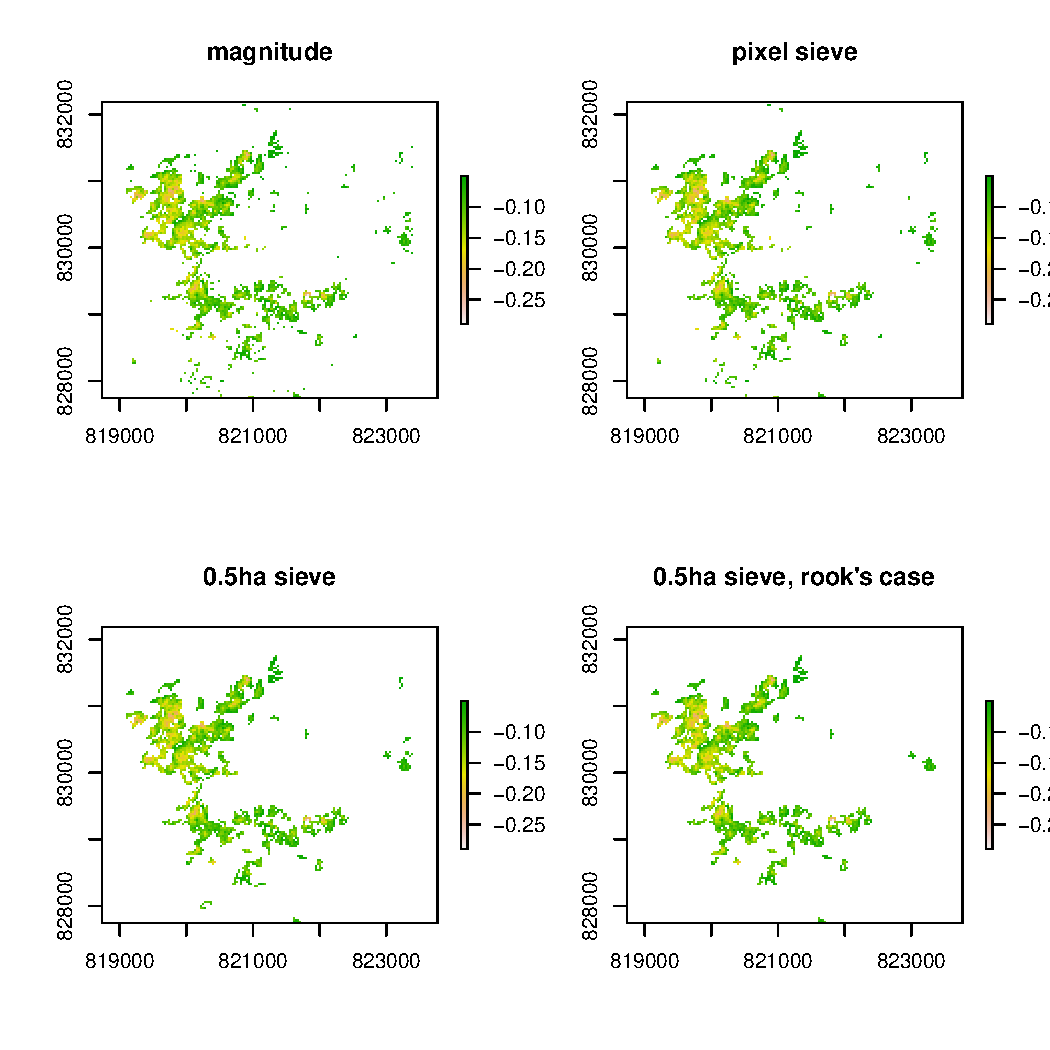
\includegraphics[width=\maxwidth]{figure/areaSieve-rook} 
\begin{kframe}\begin{alltt}
\hlkwd{par}\hlstd{(op)}
\end{alltt}
\end{kframe}
\end{knitrout}


Once we have applied the desired filters and sieves to our bfm magnitude raster, we may want to calculate area statistics. This can be done with another simple function: \code{clumpSize}. This function is also based on the \code{raster::clumps} function and computes the size of each pixel clump and assigns that value back to each pixel in that clump. As in \code{areaSieve}, the queen's and rook's cases can also apply by adjusting the \code{directions} argument.

\begin{knitrout}
\definecolor{shadecolor}{rgb}{0.969, 0.969, 0.969}\color{fgcolor}\begin{kframe}
\begin{alltt}
\hlstd{changeSize_queen} \hlkwb{<-} \hlkwd{clumpSize}\hlstd{(magn09_areasieve)}
\hlstd{changeSize_rook} \hlkwb{<-} \hlkwd{clumpSize}\hlstd{(magn09_areasieve,} \hlkwc{directions} \hlstd{=} \hlnum{4}\hlstd{)}
\hlcom{# compare}
\hlstd{op} \hlkwb{<-} \hlkwd{par}\hlstd{(}\hlkwc{mfrow} \hlstd{=} \hlkwd{c}\hlstd{(}\hlnum{1}\hlstd{,} \hlnum{2}\hlstd{))}
\hlkwd{plot}\hlstd{(changeSize_queen,} \hlkwc{col} \hlstd{=} \hlkwd{bpy.colors}\hlstd{(}\hlnum{50}\hlstd{),} \hlkwc{main} \hlstd{=} \hlstr{"Clump size: Queen's case"}\hlstd{)}
\hlkwd{plot}\hlstd{(changeSize_rook,} \hlkwc{col} \hlstd{=} \hlkwd{bpy.colors}\hlstd{(}\hlnum{50}\hlstd{),} \hlkwc{main} \hlstd{=} \hlstr{"Clump size: Rook's case"}\hlstd{)}
\end{alltt}
\end{kframe}
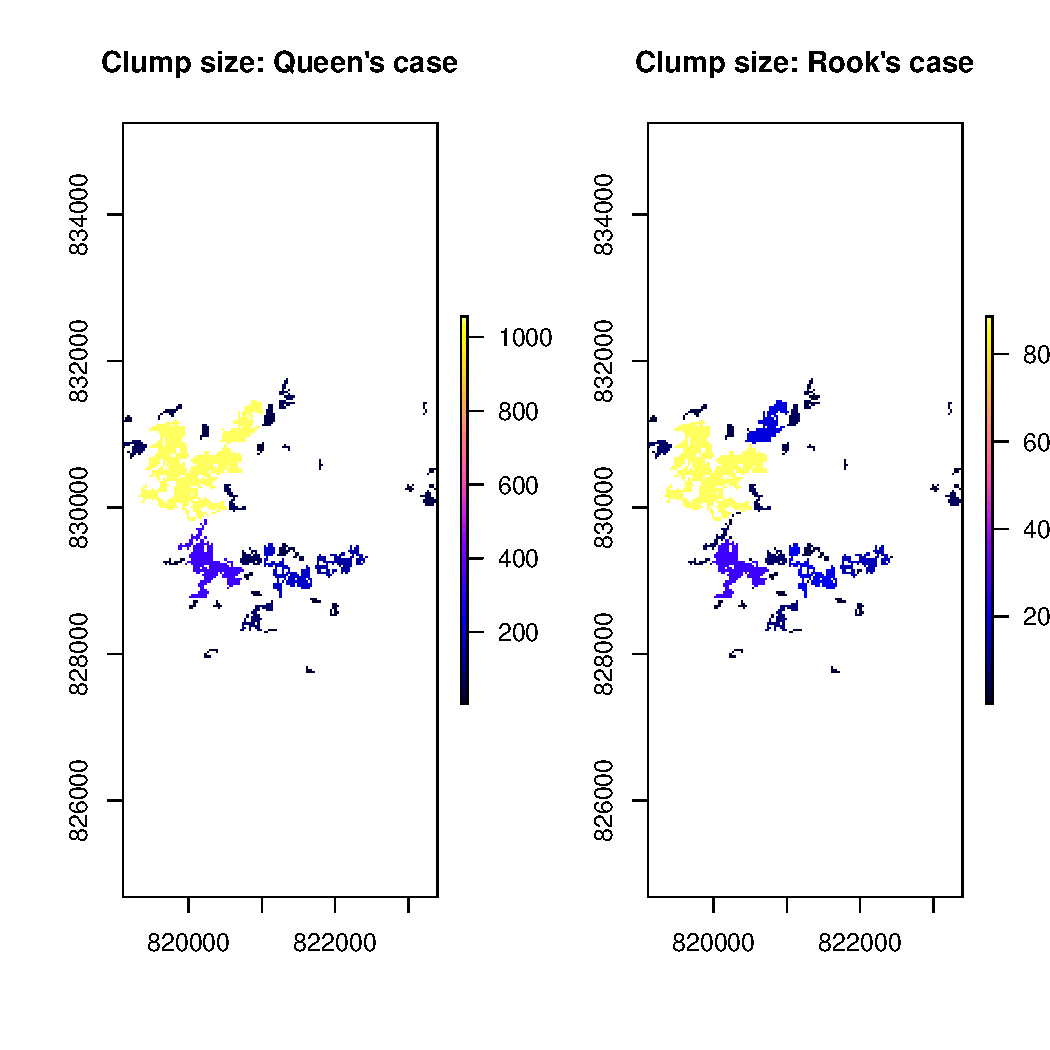
\includegraphics[width=\maxwidth]{figure/clumpSize} 
\begin{kframe}\begin{alltt}
\hlkwd{par}\hlstd{(op)}
\end{alltt}
\end{kframe}
\end{knitrout}


These clump sizes are in number of pixels, which might not be very useful when communicating our results to other parties. The \code{f} argument in \code{clumpSize} allows us to convert these to a useful area measure. In the case of Landsat, we know that each pixel covers 900$m^2$, and that one hectare equals 10000$m^2$. \code{clumpSize} can perform this conversion if a value for \code{f} is supplied.

\begin{knitrout}
\definecolor{shadecolor}{rgb}{0.969, 0.969, 0.969}\color{fgcolor}\begin{kframe}
\begin{alltt}
\hlstd{changeSize} \hlkwb{<-} \hlkwd{clumpSize}\hlstd{(magn09_areasieve,} \hlkwc{f} \hlstd{=} \hlnum{900}\hlopt{/}\hlnum{10000}\hlstd{)}
\hlkwd{plot}\hlstd{(changeSize,} \hlkwc{col} \hlstd{=} \hlkwd{bpy.colors}\hlstd{(}\hlnum{50}\hlstd{),} \hlkwc{main} \hlstd{=} \hlstr{"Clump size (hectares)"}\hlstd{)}
\end{alltt}
\end{kframe}
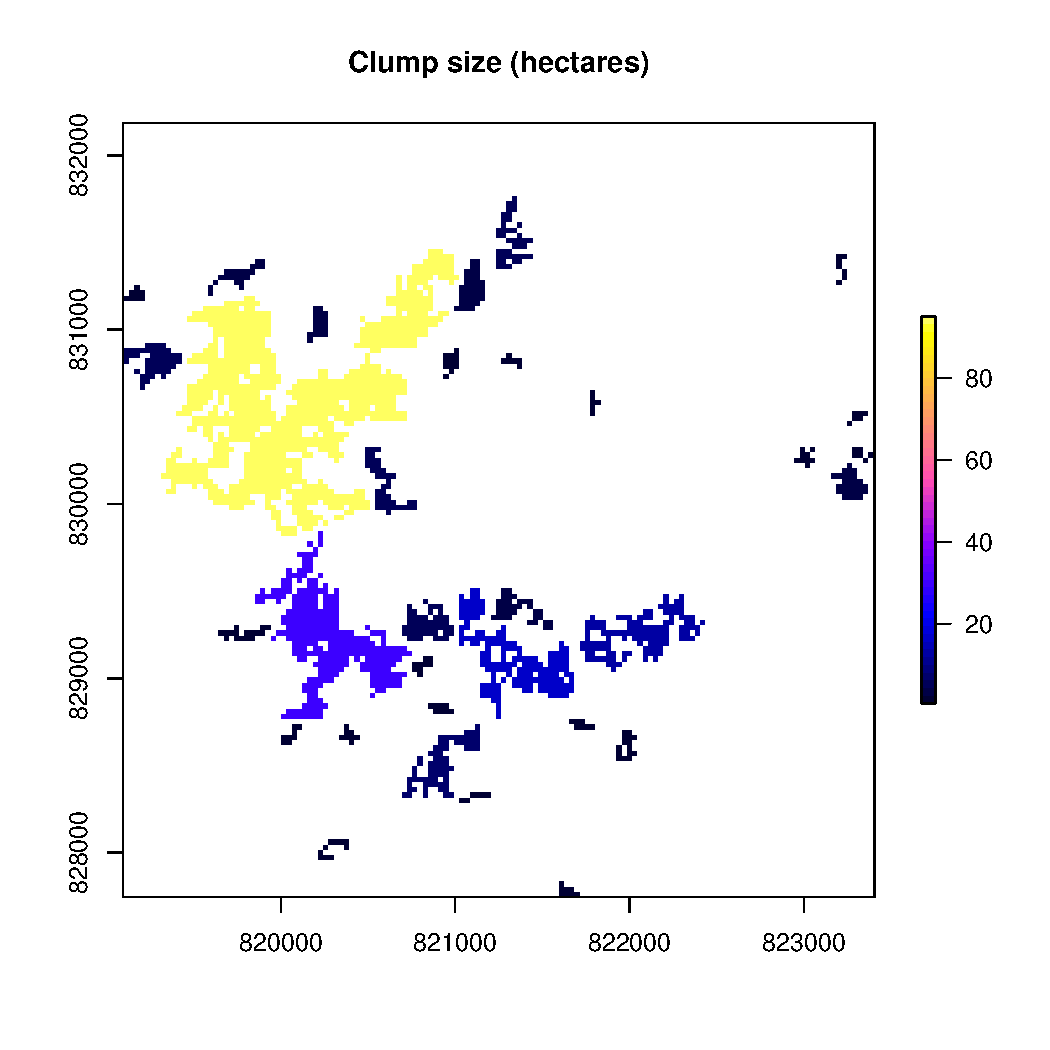
\includegraphics[width=\maxwidth]{figure/clumpSize-ha} 

\end{knitrout}


In order to calculate statistics of the changed area, it may be tempting to simply run \code{raster::summary}. But this function will produce misleading results, as \emph{each pixel} has been assigned the value of its respective clump size (rather than representing each clump as a singular object, as would be the case with a SpatialPolygons object). To circumvent this, a \code{stats} argument is included in \code{clumpSize}, which outputs an additional summary table based on clumps rather than on individual pixels. If \code{stats=TRUE}, rather than outputting a single raster layer, \code{clumpSize} returns a list with 2 objects: (1) a raster layer as above; and (2) a summary table (matrix) showing mean, min, and all quartiles of the clump sizes.

\begin{knitrout}
\definecolor{shadecolor}{rgb}{0.969, 0.969, 0.969}\color{fgcolor}\begin{kframe}
\begin{alltt}
\hlstd{changeSize} \hlkwb{<-} \hlkwd{clumpSize}\hlstd{(magn09_areasieve,} \hlkwc{f} \hlstd{=} \hlnum{900}\hlopt{/}\hlnum{10000}\hlstd{,} \hlkwc{stats} \hlstd{=} \hlnum{TRUE}\hlstd{)}
\hlkwd{print}\hlstd{(changeSize}\hlopt{$}\hlstd{stats)}
\end{alltt}
\begin{verbatim}
##         clump size
## Mean         6.266
## Min.         0.540
## 1st Qu.      0.720
## Median       1.215
## 3rd Qu.      3.735
## Max.        95.040
\end{verbatim}
\end{kframe}
\end{knitrout}


We can say that based on our analysis, the average size of change units in Tura in 2009 is estimated to be 6.3 hectares. In this case, the minimum is not suprising, since we had already applied an area sieve using 0.5 hectares as our threshold.

\end{document}
